% load the document class KOMA-Script Report
\documentclass[	
		a4paper,			% Papierformat waehlen
		12pt,				% Schriftgroesse
%		BCOR5mm,			% Bindungskorrektur
%		draft,				% Randueberschreitungen werden schwarz markiert
%		DIV13,				% Unterteilung des Blatts in DIVxx - xx Teile              OBSOLETE
						% Je kleiner die Zahl umso groesser die Raender
						% Um Optimale Anpassung zu erhalten : DIVcalc + \typearea...
%		BCOR5mm,			% Bindekorrektur BCORXmm - Xmm breit                       OBSOLETE
		%pointlessnumbers,		% KEIN ZWEITER PUNKT IN DER NUMMERIERUNG DER ÜBERSCHRIFTET 2.2 statt 2.2.	
%
%      KOPF/FUSSZEILE
%		headinclude,			% Head gehoert mit zum Textblock/auskommentiert im Seitenrand
		headsepline,			% Trennlinie zwischen Kopf und Text, schaltet automatisch 
						% headinclude mit ein
%		footinclude,			% wie Head nur Foot
%		footsepline,			% wie headsepline
%
%      LAYOUTPARAMETER
%		twocolumn,			% Zweispaltige Texte
		onecolumn,			% Einspaltig
%		twoside,			% Zweiseitiger Druck re -li sind gespiegelt vom Satzspiegel
		oneside,			% Einseitig
%		openright,			% Sollte bei zweiseitigem Druck eignestellt werden
%		cleardoublestandard		% Alles fuer 2Seitige mit openright: Kolumnentitel linke Seite
%		cleardoubleplain		% nur Seitenzahlen linke Seite
%		cleardoubleempty		% linke Seite ganz leer
%		chapterprefix,			% Kapitel wir zu beginn eines Kapitels ausgegeben
%		appendixprefix,			% Anhang wird vor Kapiteln im Anhang ausgegeben
		headings=normal,		% kleine ueberschriften, oder small-, oder big-headings.
						% Standard ist Big
%
%	TABELLENEIGENSCHAFTEN
		captions=tableheading,		% Um richtigen Abstand fuer Ueberschrift zu erhalten, 
						% Ueberschrift wird genommen
%
%	VERZEICHNISEINSTELLUNGEN
%		tocleft,			% Setzt das Inhaltverzeichnis nicht eingerueckt nach links
%		liststotoc,			% Abb.- und Tab.Verzeichnisse ins Inhaltsverzeichnis
%		liststotocnumbered, 		% wie liststotoc nur mit Gliederungspunktangabe
%		bibtotoc,			% Literaturverzeichnis ins Inhaltverzeichnis
%		bibtotocnumbered,		% s.o. nur mit Gliederungsebene
%		idxtotoc,			% Eintrag ins Inhaltsverzeichnis fue Index
%		openbib,			% Veraendert aussehen des Lit.-Verzeichnisses
%	Language
%		ngerman,			% to pass as standard to all packages
%halfparskip,                                         % Europäischer Satz: Abstand zwischen Absätzen
%	abstracton,																					 % Spezielle Formatierung, die erlaubt, dass die
																											 % Zusammenfassung vor dem Inhaltsverzeichnis steht
	%draft,		 % Es handelt sich um eine Vorabversion	
%	final		 % Es handelt sich um die endgültige Version
]{scrreprt}

% load packages for european, espacially german users

\usepackage[T1]{fontenc}			% Schriften fuer Europaeische Zeichen passend Kodiert
\usepackage[utf8]{inputenc}        		% Eingabe von Umlauten, ss usw. - 
						% utf8: kann nicht jeder Editor speicher, aber plattformuebergreifend
						% latin1: Unix, VMS, Windows
						% ansinew: Windows
						% latin9: wie latin1, jedoch mit Eurozeichen
						
\usepackage[					% Passt Konventionen an Sprache an
	     english, 
	     ngerman				% ngerman: Neue Deutsche Rechtschreibung
	    ]{babel}				% z.B. UKenglish, USenglish, canadian, german, austrian, naustrian
	    
%\usepackage[latin1]{inputenc}                   % direkte Umlauteingabe (ä statt "a)
                                                % latin1/latin9 für unixoide Systeme
                                                % (latin1 ist auch unter Win verwendbar)
                                                % ansinew für Windows
                                                % applemac Macs
                                                % cp850 OS/2
\usepackage{times}              	        % Schriften Paket
\usepackage{array,ragged2e} 			% Wichtig für Abstandsformatierung
%---------------------------------------------------------------------------------------------------
\usepackage{cmbright}                                  % serifenlose Schrift als Standard
                                                       % + alle für TeX benötigten mathematischen
                                                       %   Schriften einschließlich der AMS-Symbole
\usepackage[scaled=.90]{helvet}                        % skalierte Helvetica als \sfdefault
\usepackage{courier}                                   % Courier als \ttdefault
%---------------------------------------------------------------------------------------------------
%\usepackage[automark]{scrpage2}                        % Anpassung der Kopf- und Fußzeilen
\usepackage{xspace}                                    % Korrekter Leerraum nach Befehlsdefinitionen
\usepackage{setspace}				  % Dieses Package brauchen wir für den 				
\usepackage[pdftex]{graphicx}
\usepackage[absolute,overlay]{textpos}         

%\usepackage{natbib}                                    % Neuimplementierung des \cite-Kommandos
\usepackage{bibgerm}       				 % Deutsche Bezeichnungen
\usepackage[final]{pdfpages}                           % include pages of external PDF documents

%\usepackage{makeidx}					% Paket zur Erstellung eines Stichwortverzeichnisses
%\makeindex						 % Automatische Erstellung des Stichwortverzeichnis
%\usepackage[intoc,
%						german,
%						prefix]{nomencl}
%\makenomenclature
	    
%\hyphenation{}					% Trennung von Woertern falls nicht automatisch korrekt erkannt
%\usepackage{icomma}				% Bei deutscher Schreibweise, damit keine

%\usepackage[scaled=0.66]{luximono}		% Schrift fuer Typewriter - Quellcode ~8pt
				

% Fuer optimale Anpassung des Satzspiegels
%\typearea[current]{calc}			% Bestimmt Rasterzahl aus Schriftgroesse und Anzahl der 		
						% Zeichen/Woerter pro Zeile

% FUSS UND KOPFZEILENANPASSUNG
%\pagestyle{plain}				% empty: Keine Kopf/Fusszeile
						% plain: Seitenzahl am Fussende
						% headings: aktiviert lebende Kolumnentitel (Kapitel im Kopf)
						% myheadings : eigene Kopf- fußzeilen
						% fancy: Erlaubt die Verwendung der in dem Paket "fancyhdr" 
						% definierten Befehle zur Erstellung eigener Kopf- und Fußzeilen

%%error
% scrpage2 ist obsolete!
%\usepackage[
%	    automark				% takes the chapter variant
%	   ]{scrpage2}				% Fuer eigene Kopf/Fusszeilen, ermoeglicht. 
% stattdessen scrlayer-scrpage:

\usepackage{scrlayer-scrpage}
\pagestyle{scrheadings} %, scrplain}
\clearscrheadings				% clear old header style
\clearscrplain					% clear plain header style
\clearscrheadfoot				% clear foot style
\automark[chapter]{chapter}
\ohead{\pagemark}				% beide Außenseiten des Headers --Seitenzahl
\ihead{\headmark}				% beide Innenseiten Headers -- Chapter

%\chead						% zentriert 
%\lehead					% left even
%\cehead
%\rehead
%\lohead					% left odd
%\cohead
%\rohead
%%


%\lehead{\leftmark}
%\lohead{\rightmark}
%\ofoot[\pagemark]{}				% auf plain seiten Seitenzahl außen
									
% Schriftfamilien Laden
\usepackage{lmodern}				% Laedt die Schriftart Latin-Modern fuer Text
\usepackage{textcomp}
%\usepackage{courier}
%\rmfamily
%\sffamily
%\ttfamily
%\renewcommand{\rmdefault}{
%			  pbk	% Bookman
%			  phv	% Helvetica
%			  cmr	% CM Roman
%			  ppl	% Palatino
%			  ptm	% Times Roman
%			  pag	% Avant Garde
%			  pcz	% Zapf Chancery
%			 }
%\renewcommand{\familydefault}{\sfdefault}

% Alternativ Schriftart (Textshchrift) ändern über usepackage:
%\usepackage{
%	    mathpazo	% Palatino
%	    mathptmx	% Times
%	    avant	% Avant Garde
%	    courier	% Courier
%	    chancery	% Zapf Chancery
%	    bookman	% Bookman
%	    newcent	% New Century Schoolbook
%	    charter	% Charter
%	    helvet	% Helvetica
%} 
%\usepackage[scaled=0.92]{helvet}		% Helvetica, ist größer als Times und sollte bei verwendung beider skaliert werden.

% Im Dokument wechslen:
%\fontfamily{pbk}\selectfont

\usepackage[
	    babel,
%	    german=guillemets,  		% franz. <<  >>
	    german= quotes,			% deutsche Anfuehrungszeichen "
	   ]{csquotes}				% Laden der richtigen Anfuehrungszeicehn fuer deutsche sprache
						% = quotes fuer englische sprache



	   
%\usepackage{setspace}				% Fuer Abstaende im Dokument
%\onehalfspacing				% aendert Zeilenabstand auf 1 1/2
									
%\usepackage{microtype}				% optischer Randausgleich in PDF's
									% ungeeignet fuer internettexte o.ae.	
	   
%\usepackage[					% Papierformate auf denen gedruckt werden soll
%		a0,b0,
%		a1,b1,
%		a2,b2,
%		a3,b3,
%		a4,b4,
%		a5,b5,
%		a6,b6,
%		letter,
%		legal,
%		executive,
%		center,				% zentrierter druck
%		landscape,			% querformat
%		]{crop}
	 
									
\usepackage[a4paper]{geometry}			% Anpassung von Seitenraender per Hand
\geometry{					% Wenn Zweiseitig-> left->inner : right->outer	
	    top=2cm, 				% Weitere Moeglichkeiten: height - Texthoehe, width - Textbreite
	    bottom=5cm,
	    inner=2cm,
	    outer=3cm
         }	

\setlength{\headheight}{1.5cm}
\setlength{\voffset}{0.5cm}


\usepackage[					% To set Text at a specific 
		absolute,			% absolute - absolute position on the page
		overlay,			% overlay - if using absolute option text is placed below other things
%		showboxes,			% showboxes - shows boxes around the text
%		noshowtext,			% noshowtext - just show the box if it is on
%		verbose,			% verbose - package writing things to output like calculations
%		quiet,				% quiet turns this off : verbose = default
	    ]{textpos}

\usepackage[
	    hyperref 	= false,		% switch off hyperref hack
	    float 	= true,			% switch off float hack
	    listings 	= true,  		% switch off listings hack
	   ]{scrhack}				% to get rid off the warning @addtocbasic

	   
%\usepackage{anyfontsize} % hilft gegen font shape not available, was wegen \DeclareMathSizes auftreten kann
\usepackage{relsize}                            % für größere und kleinere Gleichungen über den Befehl \mathlarger bzw. \mathsmaller, auch \textlarger und \textsmaller

\usepackage{lscape}

%---------------------------------------------------------------------------------------------------
% Anpassung der Parameter, die TeX bei der Berechnung der Zeilenumbrüche verwendet:
%---------------------------------------------------------------------------------------------------
\tolerance 1414
\hbadness 1414
\emergencystretch 1.5em
\hfuzz 0.3pt
\widowpenalty=10000
\vfuzz \hfuzz
\raggedbottom

\usepackage{color}				% to use colors, espacially for source codes
\usepackage[%
%	    table				% Zum automatischen Laden des Pakets colortbl - fuer Tabellen
	   ]{xcolor}				% for Hyperref package, that one can say red than rgb values

	   
	   
\definecolor{mygreen}{rgb}{0,0.6,0}
\definecolor{forestgreen}{rgb}{0.0, 0.27, 0.13}
\definecolor{mygray}{rgb}{0.5,0.5,0.5}
\definecolor{mymauve}{rgb}{0.58,0,0.82}
\definecolor{lila}{rgb}{0.6, 0.4, 0.8}
\definecolor{lavendel}{rgb}{0.75, 0.58, 0.89}
\definecolor{applegreen}{rgb}{0.55, 0.71, 0.0}
\definecolor{azure}{rgb}{0.0, 0.5, 1.0}
\definecolor{yellow}{rgb}{0.99, 0.93, 0.0}
\definecolor{brown}{rgb}{0.59, 0.29, 0.0}
\definecolor{cinnamon}{rgb}{0.82, 0.41, 0.12}
\definecolor{pumpkin}{rgb}{1.0, 0.46, 0.09}
\definecolor{pink}{rgb}{0.91, 0.25, 0.78}

\definecolor{DOGGYbg}{RGB}{80,90,100} %HAW Color
\definecolor{DOGGY}{RGB}{26,60,116} % HAW Color 2
\definecolor{lgray}{RGB}{240,240,240} %HAW Color
\definecolor{darkgreen}{RGB}{50,150,50} %HAW Color

\definecolor{brightgray}{RGB}{230,230,230}

\newcommand{\boxColorForOne}{black}
\newcommand{\boxColorForZero}{lightgray}
\newcommand{\boxColorForSqrt}{green}

\newcommand{\textColorForOne}{white}
\newcommand{\textColorForZero}{black}
\newcommand{\textColorForSqrt}{black}

\newcommand{\boxHeightL}{7}
\newcommand{\boxWidthL}{7}
\newcommand{\boxHeightS}{7}
\newcommand{\boxWidthS}{7}
\newcommand{\boxWidthWide}{7}
\newcommand{\boxHeightHigh}{7}



\newcommand{\myboxOnePos}{\colorbox{\boxColorForOne}{\makebox(\boxWidthL,\boxHeightL){\textcolor{\textColorForOne}{}}}}
\newcommand{\myboxOneNeg}{\colorbox{\boxColorForOne }{\makebox(\boxWidthL,\boxHeightL){\textcolor{\textColorForOne}{-}}}}
\newcommand{\myboxZero}  {\colorbox{\boxColorForZero}{\makebox(\boxWidthL,\boxHeightL){\textcolor{\textColorForZero}{}}}}
\newcommand{\myboxSqrtPos}{\colorbox{\boxColorForSqrt}{\makebox(\boxWidthL,\boxHeightL){\textcolor{\textColorForSqrt}{}}}}
\newcommand{\myboxSqrtNeg}{\colorbox{\boxColorForSqrt}{\makebox(\boxWidthL,\boxHeightL){\textcolor{\textColorForSqrt}{-}}}}

\newcommand{\myBlackBox}{\colorbox{black}{\makebox(\boxWidthS,\boxHeightS){\textcolor{\textColorForSqrt}{}}}}
\newcommand{\myGrayBox}{\colorbox{gray}{\makebox(\boxWidthS,\boxHeightS){\textcolor{\textColorForSqrt}{}}}}
\newcommand{\myLightgrayBox}{\colorbox{lightgray}{\makebox(\boxWidthS,\boxHeightS){\textcolor{\textColorForSqrt}{}}}}
\newcommand{\myDarkgrayBox}{\colorbox{darkgray}{\makebox(\boxWidthS,\boxHeightS){\textcolor{\textColorForSqrt}{}}}}

\newcommand{\myBlackBoxHigh}{\colorbox{black}{\makebox(\boxWidthS,\boxHeightHigh){\textcolor{\textColorForSqrt}{}}}}
\newcommand{\myBlackBoxWide}{\colorbox{black}{\makebox(\boxWidthWide,\boxHeightS){\textcolor{\textColorForSqrt}{}}}}
\newcommand{\myLightgrayBoxHigh}{\colorbox{lightgray}{\makebox(\boxWidthS,\boxHeightHigh){\textcolor{\textColorForSqrt}{}}}}
\newcommand{\myLightgrayBoxWide}{\colorbox{lightgray}{\makebox(\boxWidthWide,\boxHeightS){\textcolor{\textColorForSqrt}{}}}}

\usepackage{tcolorbox} 

\newtcolorbox{mytextbox}[1]{%
    tikznode boxed title,
    enhanced,
    arc=0mm,
    interior style={white},
    attach boxed title to top left= {xshift=0.5cm, yshift=-\tcboxedtitleheight/2},
    fonttitle=\bfseries,
    colbacktitle=white,coltitle=black,
    boxed title style={size=normal,colframe=gray,boxrule=0pt},
    title={#1}}
\usepackage[%
%	    leqno,				% Nummern linksbuendig
%	    reqno,				% Nummern rechtsbuendig (Standard)
%	    fleqn,				% Gleichungen linksbuendig statt zentriert
	   ]{amsmath}
\usepackage{amsfonts}				% Um Zahlenraeume richtig darzustellen
\usepackage{mathtools}


% Betragsstriche über \abs, Doppelbetragsstriche über \norm
\DeclarePairedDelimiter\abs{\lvert}{\rvert}%
\DeclarePairedDelimiter\norm{\lVert}{\rVert}%

\usepackage[%
	    thinlines,				% dünne linien
%	    thicklines,				% dicke linien
	   ]{easybmat}				% For Matrices with dottet lines between fields, horizontal or vertical
%\usepackage{MnSymbol}				% Zusaetzliche Zeichen
\usepackage{trsym}				% Fuer Laplace-Fourier-Symbole
\usepackage{mathrsfs}				% Fuer Matheschrift
\usepackage{xfrac}
\usepackage{nicefrac}
\usepackage{esint}
%\usepackage{exscale} % lässt Klammern in Gleichungen verschwinden!!
%\DeclareMathSizes{10.95}{30}{15}{15} % 10.95 für 11pt in documentclass

\def\mathunderline#1#2{\color{#1}\underline{{\color{black}#2}}\color{black}}

\usepackage{soul}

\usepackage[%				
%	    group-separator 	= {.}, 		% group-seperator={,} -> 1,345,234.23
%   	    round-mode 		= places,		% round-mode= places(2digits), figures(1digit)
%	    round-precision 	= 3,		% round-precision= x , xdigits are rounded to
	    binary-units 	= true,		% Laden von \byte \bit, \kibi usw. (false default)
	    locale 		= DE,		% lacale= DE, uses german
	    per			= slash,
	    alsoload            = binary,
%	    loctolang		={
%				  UK:english, 
%				  DE:ngerman
%		      		 },		% loctolang={USA:USenglish,DE:ngerman}, if language changed in document
	    detect-all				% detect-all : uses the text options not the math mode to set the letters/numbers
	   ]{siunitx}

\usepackage{graphicx} 				% für Grafik-Einbindung
%\usepackage{subfigure}				% Für Untergrafiken, wenn eine eigene Bildunterschrift erwuenscht
\usepackage{subcaption}
\usepackage[hypcap=false]{caption}				% für Captions bei Grafiken ohne figure Umgebung wie in Minipage nötig
\usepackage[%
	    update				% if pdf conversion is older than eps file, new conversion is done
	   ]{epstopdf}				% eps to pdf needs for pdflatex - after graphicx

%\usepackage{subfig}
\usepackage{capt-of}

%---------------------------------------------------------------------------------------------------
% Abbildungsverzeichnis
%---------------------------------------------------------------------------------------------------
%\graphicspath{{img/}}

\usepackage{tikz}
%\usepackage{background}
\usetikzlibrary{thedecorations, arrows,shapes, automata, positioning, calc, backgrounds, decorations.pathreplacing}


\newcommand{\tikzmark}[1]{\tikz[overlay, remember picture] \coordinate (#1);}

\tikzset{node/.style={draw,shape=circle}}
\newcommand{\order}[2][th]{\ensuremath{{#2}^{\mathrm{#1}}}}
\usepackage{multirow}				% Fuer Mehrzeilige Zellen
\usepackage{multicol}
%\usepackage{array}					% Festlegen von Breiten, Präfixe, Suffixe
% see also package siunitx - damit Spalten mit Zahlen auf bestimmte Länge ausgerichtet werden
\usepackage{tabularx}				% Zum festlegen der Gesamtbreite der Tabelle & verwenden von X fuer 
									% variable Spaltenbreite
%\usepackage{longtable}				% Tabelle ueber mehr als eine Seite
\usepackage{ltxtable}				% longtable + tabularx eigenschaften

%\usepackage{rotating}				% Querformat der Tabelle
									% !!! Vorsicht !!!
									% tablecaptionabove wird nicht ausgewertet,
									% Einfuegen von \vskip\abovecaptionskip --> Nur unter KOMA Script
\usepackage{ctable}					% For tables with footnote under the table directly


\setlength{\arraycolsep}{0.4pt}
\delimitershortfall=0pt % Höhereduzierung der Klammern von Matrizen gegenüber dem Inhalt

\usepackage{tabu} % fuer farbige Zeilen in Tabellen
\usepackage[  % Packet ist jetzt glossaries-extra statt glossaries - keine Ahnung, ob die es die auskommentierten Optionen gibt!
	    xindy,%={language=german-modern, codepage=utf8},
	    automake,				
	    numberedsection,
%	    toc,      				% Fügt Eintrag ins Inhaltsverzeichnis hinzu, defualt false
	    nonumberlist,			% keine Ausgabe der Seitenzahlen
%	    nowarn,				% unterdrückt alle warungen des pakets
%	    nomain,				% kein hauptglossary wird erzeugt, acronym oder newglossary um Einträge zu erzeugen
%	    sanitize={%				% unterdrückt die keys für einträge oder fügt sie hinzu
%	    name        = false,%
%	    description = false,%
%	    symbol      = false},%
%	    translate = true,			% zur übersetzung von einträgen - siehe doku, default false
	    hyperfirst = true,			% erzeugt hyperlink zum glossar bei erster verwendung, default true
%	    hyper = false,			% Hyperlinks ausschalten
%	    numberline,				% Eintrag ins toc mit Nummerierung
%	    section=section,			% in welcher ebene der eintrag, default chapter if loaded sonst section
%	    style = long,			% default list, sonst: long, super, tree
%	    nolong,				% pakete für longtable werden nicht geladen und befehle nicht definiert
%	    nosuper,				% supertabular wird nicht geladen, pakete nicht definiert
%	    nolist,				% list wird nicht geladen definiert
%	    notree,				% gloassrytree wird nicht geladen definiert
%	    nostyles,				% keine styles werden geladen, eigene definieren
%	    counter = page,			% page default, or any other counter
%	    sort = def,				% def - sortiert nach definition, standard(default)-sortiert nach sort key, sonst name, use - sortieren nach reihenfolge wie sie im dokument vorkommen
%	Acronym options
%	    acronym,  				% Seperate Liste für Acronyme zum Glossary, default - false
%	    acronymlist={},			% wenn mehr als eine abkürzungsliste, muss diese hier mit angegeben werden damit das glossary als acronym behandelt wird
%	    description,			% erlaubt eine zusätzliche beschreibung
%	    footnote,				% schreibt die long version als fußnote bei erster nutzung
%	    smallcaps,				% acronyme werden als kapitelchen angezeigt
%	    smaller,				% kleinere schrift, laden von relsize für befehl textsmaller erforderlich
%	    dua,				% langform wird immer ausgegeben
	    shortcuts,				% um selbe befehle wie acronym paket zu haben
	   ]{glossaries-extra}		


\GlsSetXdyCodePage{duden-utf8}

% sorgt dafür, dass die Erklärungen alle gleich eingerückt sind
\setglossarystyle{long}
\renewcommand{\glsnamefont}[1]{\textbf{#1}}

% Bachlorarbeit.gls erzeugen:
% $ cd Bachelorarbeit
% $ makeglossaries "Bachelorarbeit"

\makeglossaries 

\newabbreviation{1d-dft}{1D-DFT}{eindimensionale diskrete Fouriertransformation}
\newabbreviation{1d-dftn}{1D-DFT}{eindimensionalen diskreten Fouriertransformation}
\newabbreviation{2d-dft}{2D-DFT}{zweidimensionale diskrete Fouriertransformation}
\newabbreviation{2d-dftn}{2D-DFT}{zweidimensionalen diskreten Fouriertransformation}

\newabbreviation{adc}{ADC}{Analog Digital Converter}
\newabbreviation{adu}{ADU}{Analog Digital Umsetzer}
\newabbreviation{amr}{AMR}{anisotroper magnetoresistiver Effekt}
\newabbreviation{amr2}{AMR}{anisotropen magnetoresistiven Effekt}
\newabbreviation{asic}{ASIC}{Application Specific Integrated Circuit, \textit{dt.: Anwendungsspezifischer Integrierter Schaltkreis}}

\newabbreviation{dac}{ADC}{Digital Analog Converter}
\newabbreviation{dau}{ADU}{Digital Analog Umsetzer}
\newabbreviation{dct}{DCT}{diskrete kosinus Transformation}
\newabbreviation{dft}{DFT}{diskrete Fouriertransformation}

\newabbreviation{idft}{IDFT}{inverse diskrete Fouriertransformation}
\newabbreviation{isar}{ISAR}{Integrated Sensor Array}

\newabbreviation{ft}{FT}{Fouriertransformation}
\newabbreviation{fft}{FFT}{Fast Fouriertransformation}

\newabbreviation{lsb}{LSB}{Least Significant Bit}

\newabbreviation{msb}{MSB}{Most Significant Bit}

\newabbreviation{ram}{RAM}{Random Access Memory}

\newabbreviation{tmr}{TMR}{tunnelmagnetoresistiver Effekt}
\newabbreviation{tmr2}{TMR}{tunnelmagnetoresistiven Effekt}



\glsaddall

\setlength\LTleft{0pt}
\setlength\LTright{0pt}
\setlength\glsdescwidth{0.8\hsize}


% Hyperref for PDFLATEX with links    
\usepackage[
	    draft 	= false,			% all hypertext options are turned off
	    final 	= true, 			% all hypertext options are turned on
	    raiselinks 	= true,				% Allow links to reflect real height - e.g. with pictures
	    breaklinks	= false,			% false=Do not break a line within a link
	    backref	= false,			% false=no backlinks in the bibliography
	    pagebackref = false,			% false=no pagebacklinks in bibliography
%	    linktocpage = true,				% true=makes page-no linked and not text in TOC,LOF and LOT
	    linktoc	= all,
%			  none,
%			  section,
%			  page,
	    colorlinks	= false,			% true=Colors the text of links and anchors
%	    linkcolor 	= red, 				% Color for normal internal links.
%	    anchorcolor = black, 			% Color for anchor text.
%	    citecolor 	= green, 			% Color for bibliographical citations in text.
%	    filecolor 	= cyan, 			% Color for URLs which open local files.
%	    menucolor 	= red,				% Color for Acrobat menu items.
%	    runcolor 	= filecolor,			% Color for run links (launch annotations).
%	    allcolors 	= red,				% Set all color options (without border and field options).
	    urlcolor 	= blue,				% Color for linked URLs.
%	    allbordercolors  =red,			% Set all colors
%	    citebordercolor =green,			% cite color
%	    filebordercolor =cyan,			% file color
%	    linkbordercolor =red,			% link color
%	    urlbordercolor  =blue,			% url color
%	    pdfborder = 0 0 0,				% weder farbige links noch umrandung			
%	    menubordercolor =red,			% set menu color
%	    frenchlinks = 	false,			% Use small caps instead of color for links.
	    bookmarks	=	true,			% true=Bookmarks are added to the pdf
	    bookmarksopen=	false,			% false=Bookmarks not open when opening the pdf
	    bookmarksnumbered=true,			% true= Eintraege sind nummeriert
%	    pdfpagemode	=	FullScreen,		% File is opened in Full Screen
%	    pdfstartview=	fit,			% Fit size when opening pdf
	    pdfpagelabels=	true,			% true = Roemische Zahlen usw werden dargestellt,
							% false= fortlaufende nummerierung
	   ]{hyperref}
\hypersetup{hidelinks}

\usepackage{listings}					% options : basicstyle= e.g. \ttfamily
							% fontadjust=true % before load package [scaled=0.78]{luximono}
							% columns=flexible

\lstset{ %
  backgroundcolor=\color{white},   % choose the background color; you must add \usepackage{color} or \usepackage{xcolor}; should come as last argument
  basicstyle=\footnotesize,        % the size of the fonts that are used for the code
  breakatwhitespace=false,         % sets if automatic breaks should only happen at whitespace
  breaklines=true,                 % sets automatic line breaking
  captionpos=b,                    % sets the caption-position to bottom
  commentstyle=\color{mygreen},    % comment style
  deletekeywords={...},            % if you want to delete keywords from the given language
  escapeinside={\%*}{*)},          % if you want to add LaTeX within your code
  extendedchars=true,              % lets you use non-ASCII characters; for 8-bits encodings only, does not work with UTF-8
  frame=single,	                   % adds a frame around the code
  keepspaces=true,                 % keeps spaces in text, useful for keeping indentation of code (possibly needs columns=flexible)
  keywordstyle=\color{blue},       % keyword style
  language=VHDL,                 % the language of the code
  morekeywords={*,...},            % if you want to add more keywords to the set
  numbers=none,                    % where to put the line-numbers; possible values are (none, left, right)
  numbersep=5pt,                   % how far the line-numbers are from the code
  numberstyle=\tiny\color{mygray}, % the style that is used for the line-numbers
  rulecolor=\color{black},         % if not set, the frame-color may be changed on line-breaks within not-black text (e.g. comments (green here))
  showspaces=false,                % show spaces everywhere adding particular underscores; it overrides 'showstringspaces'
  showstringspaces=false,          % underline spaces within strings only
  showtabs=false,                  % show tabs within strings adding particular underscores
  stepnumber=2,                    % the step between two line-numbers. If it's 1, each line will be numbered
  stringstyle=\color{mymauve},     % string literal style
  tabsize=2,	                   % sets default tabsize to 2 spaces
  title=\lstname                   % show the filename of files included with \lstinputlisting; also try caption instead of title
  literate=
  {á}{{\'a}}1 {é}{{\'e}}1 {í}{{\'i}}1 {ó}{{\'o}}1 {ú}{{\'u}}1
  {Á}{{\'A}}1 {É}{{\'E}}1 {Í}{{\'I}}1 {Ó}{{\'O}}1 {Ú}{{\'U}}1
  {à}{{\`a}}1 {è}{{\`e}}1 {ì}{{\`i}}1 {ò}{{\`o}}1 {ù}{{\`u}}1
  {À}{{\`A}}1 {È}{{\'E}}1 {Ì}{{\`I}}1 {Ò}{{\`O}}1 {Ù}{{\`U}}1
  {ä}{{\"a}}1 {ë}{{\"e}}1 {ï}{{\"i}}1 {ö}{{\"o}}1 {ü}{{\"u}}1
  {Ä}{{\"A}}1 {Ë}{{\"E}}1 {Ï}{{\"I}}1 {Ö}{{\"O}}1 {Ü}{{\"U}}1
  {â}{{\^a}}1 {ê}{{\^e}}1 {î}{{\^i}}1 {ô}{{\^o}}1 {û}{{\^u}}1
  {Â}{{\^A}}1 {Ê}{{\^E}}1 {Î}{{\^I}}1 {Ô}{{\^O}}1 {Û}{{\^U}}1
  {œ}{{\oe}}1 {Œ}{{\OE}}1 {æ}{{\ae}}1 {Æ}{{\AE}}1 {ß}{{\ss}}1
  {ű}{{\H{u}}}1 {Ű}{{\H{U}}}1 {ő}{{\H{o}}}1 {Ő}{{\H{O}}}1
  {ç}{{\c c}}1 {Ç}{{\c C}}1 {ø}{{\o}}1 {å}{{\r a}}1 {Å}{{\r A}}1
  {€}{{\euro}}1 {£}{{\pounds}}1 {«}{{\guillemotleft}}1
  {»}{{\guillemotright}}1 {ñ}{{\~n}}1 {Ñ}{{\~N}}1 {¿}{{?`}}1
}

\usepackage[
	    official,
	    right				% Position of the Euro-Sign. verwendung: \euro oder \EUR{123,45}
	   ]{eurosym}


% Loading unit options                

\usepackage[%				
%	    group-separator 	= {.}, 		% group-seperator={,} -> 1,345,234.23
%   	    round-mode 		= places,		% round-mode= places(2digits), figures(1digit)
%	    round-precision 	= 3,		% round-precision= x , xdigits are rounded to
	    binary-units 	= true,		% Laden von \byte \bit, \kibi usw. (false default)
	    locale 		= DE,		% lacale= DE, uses german
	    per			= slash,
%	    loctolang		={
%				  UK:english, 
%				  DE:ngerman
%		      		 },		% loctolang={USA:USenglish,DE:ngerman}, if language changed in document
	    detect-all,				% detect-all : uses the text options not the math mode to set the letters/numbers
	   ]{siunitx}


\usepackage[Algorithmus]{algorithm} 			% deutsche notation im titel

% Zitate die in den Referenzen aufscheinen, aber nicht unbedingt im Text zitiert werden m�ssen
% Literatur, die mit \nocite oder \cite zitiert wird, mu� im .bib File erfasst werden!
\nocite{Guenther:2002}
\nocite{Lamport:1995}
\nocite{Goossens:2000}
\nocite{Kohm:2003}
\nocite{Hunt:2003}
\nocite{Boehm:2002}
\nocite{Schmatz:2004}
\nocite{Streitz:2005}
\nocite{HP:2004}
\nocite{Luede:2004}
\nocite{Demarco:1999}
\nocite{Kollakowski:2004}
\nocite{Dawson:2003}
\nocite{Poenicke:1988}
\nocite{Kruse:2000}
\nocite{Nilsson:1998}
\nocite{Heinsohn:1999}
\nocite{Luger:2001}
\nocite{Kuehnel:2001}
\nocite{Bigus:2001}
\nocite{Ferber:2001}
\nocite{Wooldridge:2002}
\nocite{KuroseRoss:2002}
\nocite{Vogt:2001}
\nocite{Roetzer:1999}
\nocite{P3P:2004}
\nocite{CPEX:2004}
\nocite{Duden:1997}
\nocite{Hoerauf:2001}
\nocite{Schirru:2004}
\nocite{Babic:2003}
\nocite{Luepke:2004}

	
\usepackage{bbding}					% to get cross and check symbol

\usepackage{enumerate}					% schicke Nummerierung

\usepackage{pdfpages}					% Zum Laden und einbinden von PDF-Seiten
\usepackage{pgfpages}
\usepackage{float}					% für floats (figures) in einer Minipage (geht nicht!!)
\usepackage{booktabs}					% Fuer besseres aussehen der Linien
\usepackage{framed}					% for use of newtheorem with a coloured box

\usepackage{titling}
\author{Thomas Lattmann}
\title{Chipimplementation einer zweidimensionalen Fouriertransformation für die Auswertung eines Sensor-Arrays}
\date{23.4.2018}
			
% INDEX ERZEUGEN - falls gewuenscht muessen beide direkt so eingebunden werden
%\usepackage{index}
%\makeindex

%\makenomenclature					% damit Symbolverzeichnis erzeugt wird

% Symbolverzeichnis erzeugen - lade dazu mit %%%%%%%%%%%%%%%%%%%%%%%%%%%%%%%%%%%%%%%%%%%%%%%%%%%%%%%%%%%%%%%%%%%%%%%%%%%%%%%
%  Author     : Dennis Schuethe        Date    : 28.12.2011                   %
%  Filename   : symbolpage.tex         Version : 1.0                          %
%  Information: This file will create the nomenclature and should be designed %
%               the way you want to. There are two options:                   %
%               1. Use the normal nomenclature which is given and created by  %
%                  the nomencl.sty -> see package declarations                %
%               2. To have more than one column for the nomenclature, then    %
%                  use the \begin{multicols}, but this cause a bad look,      %
%                  because the name is printed within the columns, better use %
%                  option 3                                                   %
%               3. Find the nomencl.sty and then rewrite the lines 160 and    %
%                  164 as it is shown below, then you need to add the         %
%                  \chapter*{\nomname} or \section*{\nomname} by yourself     %
%-----------------------------------------------------------------------------%
%  Changelog  :                                                               %
%  28.12.2011  opened this file                                               %
%              may the nomencl.sty could be changed by adding this as option, %
%              need to try a workaround                                       %
%  %
%%%%%%%%%%%%%%%%%%%%%%%%%%%%%%%%%%%%%%%%%%%%%%%%%%%%%%%%%%%%%%%%%%%%%%%%%%%%%%%


%157 \def\thenomenclature{%
%158  \@ifundefined{chapter}%
%159  {
%160    %\section*{\nomname}
%161    \if@intoc\addcontentsline{toc}{section}{\nomname}\fi%
%162  }%
%163  {
%164    %\chapter*{\nomname}
%165    \if@intoc\addcontentsline{toc}{chapter}{\nomname}\fi%
%166  }%

%\renewcommand{\nomname}{newname}	% New name for the nomenclature
%\chapter*{\nomname}				% Do the heading for this chapter(section)
% else			
% newpage							% only if chapter command is not used
%\begin{multicols}{2}				% Do multiple columns - use package multicol
\printnomenclature %[2cm] 			% Symbolverzeichnis mit breite xcm für symbole, std is 1cm
%\end{multicols} das Verzeichnis 
%\usepackage[
%	     intoc,					% Eintrag des Abkuerzungsverzeichnis
%	     notintoc,					% Kein Eintrag - default
%	     english,					% Ueberschrift in English (default)
%      	     german,					% in deutsch
%	    ]{nomencl}


% Loading label options               
\usepackage[ngerman]{varioref}		            	% To get automatic "see Section xy on page xx"
%\usepackage[german]{fancyref}		    		% same as varioref, except this is setting section automatically
							% Options in []-brackets:
							% language, e.g. english, ngerman - last entry is main-language
							% paren - sets the reference in ()-brackets
							% plain - no pagenumber in the reference
							% -----------------------------------------
							% standard prefixes used by fancyref:
							% sec, chap, part, fig, tab, enum, eq, fn
%\fancyrefchangeprefix{\fancyrefchaplabelprefix}{cha} 	% sets a new prefix for the label chap




% Pseudocode 			 %
\usepackage[noend]{algpseudocode}


\title[Chipimplementation einer 2D-DFT für die Auswertung eines Sensor-Arrays]{\LARGE{Chipimplementation einer zweidimensionalen Fouriertransformation für die Auswertung eines Sensor-Arrays}\\ 
\medskip \medskip \medskip \medskip \medskip  \large{Bachelorkolloquium}\\
\medskip }  

\author[TL]{Thomas Lattmann}
\date[\today]{\today} 

\begin{document}

%==================================================================================================================================
% 	Titelseite mit Thema der Arbeit, Author und Einleitung geben, was das Hauptziel ist! 
%==================================================================================================================================
%%%%%%%%%%%%%%%%%%%%%%%%%%%%%%%%%%%%%%%%%%%%%%%%%%%%%%%%%%%%%%%%%%%%%
% Define a background image for the first page
%%%%%%%%%%%%%%%%%%%%%%%%%%%%%%%%%%%%%%%%%%%%%%%%%%%%%%%%%%%%%%%%%%%%%
%\usebackgroundtemplate{\includegraphics[]{backT.pdf}}
%\usebackgroundtemplate{}
\begin{frame}[plain]
 	\titlepage
% 	\hfill
% 	\begin{center}
% 		\figw{.3}{img/hawlogo.pdf}
% 	\end{center}
\end{frame}

\usebackgroundtemplate{
\includegraphics[scale=1]{img/back.pdf}}


\begin{frame}\frametitle{Inhaltsübersicht}

Gliederung:
\begin{itemize}
 \item Einleitung
 \item Grundlagen
 \item Analyse und Entwurf
 \item Testumgebung und Evaluation
 \item Zusammenfassung und Ausblick
\end{itemize}
\end{frame}


\begin{frame}\frametitle{Einleitung: Details zur Hardware}
\begin{itemize}
 \item \SI{350}{\um} Prozess, EuroPractice
 \item Array von Magnetsensoren
 \item Sensoren, Signalverarbeitung \& Ausgabe des digitalen Nutzsignals auf einem ASIC
\end{itemize}
\begin{center}
 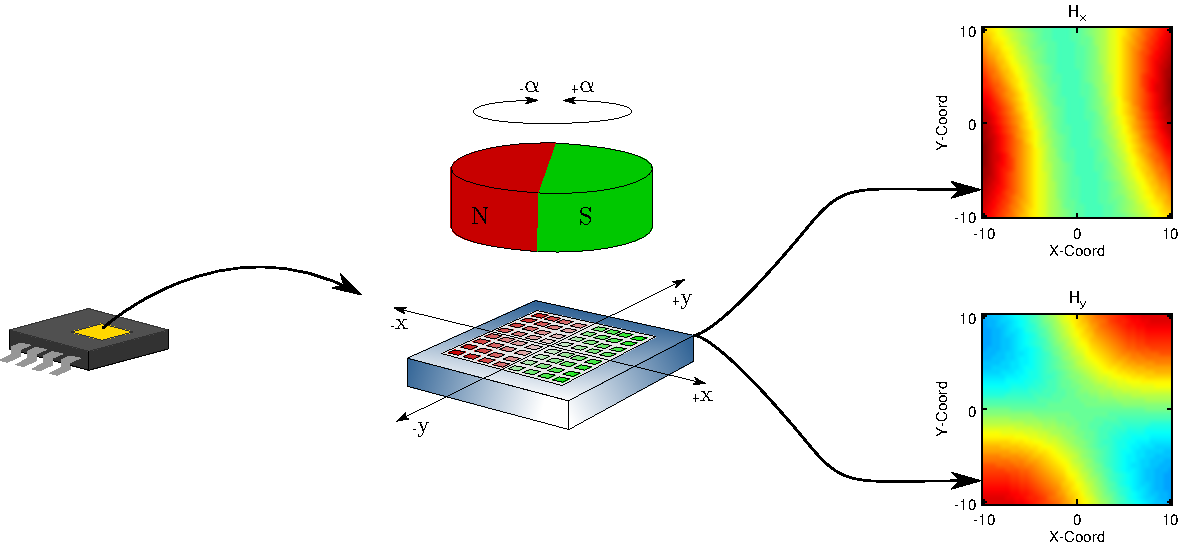
\includegraphics[width=0.6\textwidth]{img/Bilder/SensorAusgang.pdf}\\
 \tiny{Quelle: SensorAusgang.pdf, K.-R. Riemschneider + T. Schüthe}
\end{center}
\end{frame}



\begin{frame}\frametitle{Einleitung: Einordung im ISAR-Projekt}
\vspace{1cm}
 \begin{figure}[ht!]
 \centering
 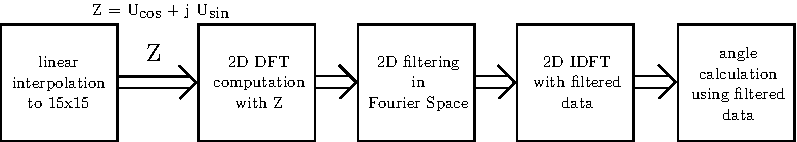
\includegraphics[width=0.8\textwidth]{img/AblaufFourier.pdf}
 %\caption{Ablauf der Signalvorverarbeitung}%~\autocite[9]{krrts2017freqfilt}}
 \label{pic:AblaufFourier}
\end{figure}
\vspace{2cm}
\begin{center}
 \tiny{Quelle: Frequency\_filtering\_and\_stray\_field\_compensation\_using\_2D-DFT\_algorithm.pdf, K.-R. Riemschneider + T. Schüthe}
\end{center}
\end{frame}



\begin{frame}\frametitle{Grundlagen}
Gliederung:
 \begin{itemize}
  \item Interpretation von Dualzahlen
  \item Komplexe Multiplikation
  \item Matrixmultiplikation
  \item DFT und IDFT
  \item 2D-DFT
 \end{itemize}
\end{frame}

% Wozu wird die 2D-DFT verwendet?


\begin{frame}\frametitle{Interpretation von Dualzahlen}
 %Alleine anhand einer binären Zahlenfolge ist nicht ersichtlich, wie sie interpretiert werden soll.\\
 \medskip
 Mögliche Arten sind:
 \begin{itemize}
  \item positive Ganzahldarstellung (a)
  \item Darstellung im Einerkomplement (b)
  \item Darstellung im Zweierkomplement (c)
  \item vorzeichenbehaftete Festkommazahlen (SQ-Format) mit u. ohne Vorkommaanteil (d)
 \end{itemize}
\medskip
\pause
Beispiel:\\
\medskip
\hspace{1cm}$1001011010100_2$
 \begin{align*}
    4096+512+128+64+16+4 &=  4820_{10}   &\textrm{(a)}\\
    - (512+128+64+16+4) & = -724_{10}   &\textrm{(b)}\\
   -4096+512+128+64+16+4 &= -3372_{10}   &\textrm{(c)}\\
   -4+0,5+0,125+0,062+0,015625+0,00390625 &= -3,29296875_{10} &\textrm{in S2Q10 (d)}
 \end{align*} 
\end{frame}

\begin{frame}\frametitle{Komplexe Multiplikation}

Komplexe Multiplikation sind 4 einfache Multiplikationen und 2 Additionen.

 \begin{align*}\label{eq:komplexe_Multiplikation}
\begin{split}
 e + jf &= (a + jb) \cdot (c + jd)\\
        &= a \cdot c + j(a \cdot d) + j(b \cdot c) + j^2(b \cdot d)\\
        &= a \cdot c - b \cdot d + j(a \cdot d + b \cdot c)
\end{split}
  \end{align*}
  
  Wenn einer der beiden Multiplikanden keinen Imaginärteil haben, reduziert sich das zu 

 \begin{align*}\label{eq:halb_komplexe_Multiplikation}
 \begin{split}
  e + jf &= a \cdot (c + jd)\\
         &= a \cdot c + j(a \cdot d)\\
 \end{split}
 \end{align*}
\end{frame}


 

% \begin{frame}\frametitle{Multiplikation im 1er-Komplemet}
% \begin{table}[ht!]
%  \centering
%  \begin{tabular}{cc|c}
%   A& B &X\\
%   \hline
%   0& 0&0\\
%   0& 1&1\\
%   1& 0&1\\
%   1& 1&0\\
%  \end{tabular}
%  \caption{Wahrheitstabelle eines XOR-Gatters. A und B sind Eingänge, X das Ausgangssignal}
%  \label{tab:xor}
% \end{table}
% \end{frame}


% \begin{frame}\frametitle{Veranschaulichung der Matrixmultiplikation}
%  \begin{center}
%  \begin{figure}[ht!]
%  \centering
% \begin{minipage}{0.2\textwidth}
%  \begingroup
%  \renewcommand*{\arraystretch}{1.1} % Zeilenabstand
%  \renewcommand*{\arraycolsep}{0.6pt} % Spaltenabstand
% 
%  \[
%     \begin{bmatrix}
%     \tikzmark{varrowtopleft} \myBlackBox  	& \myBlackBox 		& \myBlackBox 		& \tikzmark{varrowtopright} \myBlackBox \\
%                              \myLightgrayBox 	& \myLightgrayBox 	& \myLightgrayBox 	& \myLightgrayBox \\
%                              \myLightgrayBox 	& \myLightgrayBox	& \myLightgrayBox	& \myLightgrayBox \\
%     \tikzmark{varrowbottom}  \myLightgrayBox 	& \myLightgrayBox 	& \myLightgrayBox 	& \myLightgrayBox 
%    \end{bmatrix}
%  \]
%  \endgroup
%   \tikz[overlay,remember picture] {
%   \draw[->] ([yshift=1.5ex,xshift=-2ex]varrowtopleft) -- ([xshift=-2ex]varrowbottom)
%             node[midway,left] {$i$};
%   \draw[->] ([xshift=2ex,yshift=4ex]varrowtopleft) -- ([yshift=4ex]varrowtopright)
%             node[midway,above] {$k$};
% }
% \end{minipage}
% \begin{minipage}{0.1\textwidth}
%  \hspace{-.5cm}
%  \[
%   \bullet% \cdot
%  \]
% \end{minipage}
% \begin{minipage}{0.2\textwidth}
%  \begingroup
%  \renewcommand*{\arraystretch}{1.1} % Zeilenabstand
%  \renewcommand*{\arraycolsep}{0.6pt} % Spaltenabstand
%  \[
%    \begin{bmatrix}
%     \tikzmark{varrowtopleft} \myLightgrayBoxHigh & \myBlackBoxHigh & \myLightgrayBoxHigh & \tikzmark{varrowtopright} \myLightgrayBoxHigh \\
%                              \myLightgrayBoxHigh & \myBlackBoxHigh & \myLightgrayBoxHigh & \myLightgrayBoxHigh \\
%                              \myLightgrayBoxHigh & \myBlackBoxHigh & \myLightgrayBoxHigh & \myLightgrayBoxHigh \\
%     \tikzmark{varrowbottom}  \myLightgrayBoxHigh & \myBlackBoxHigh & \myLightgrayBoxHigh & \myLightgrayBoxHigh 
%    \end{bmatrix}
%  \]
%  \endgroup
%    \tikz[overlay,remember picture] {
%   \draw[->] ([yshift=1.5ex,xshift=-2ex]varrowtopleft) -- ([xshift=-2ex]varrowbottom)
%             node[midway,left] {$k$};
%   \draw[->] ([xshift=2ex,yshift=4.5ex]varrowtopleft) -- ([yshift=4.5ex]varrowtopright)
%             node[midway,above] {$j$};
% }
% \end{minipage}
% \begin{minipage}{0.05\textwidth}
%  \[
%   =
%  \]
% \end{minipage}
% \begin{minipage}{0.3\textwidth}
% \begingroup
% \renewcommand*{\arraystretch}{1.1} % Zeilenabstand
% \renewcommand*{\arraycolsep}{0.8pt} % Spaltenabstand
% \begin{align*}
%    \begin{bmatrix}
%     \tikzmark{varrowtopleft} \myLightgrayBox 	& \myBlackBox		& \myLightgrayBox 	& \tikzmark{varrowtopright} \myLightgrayBox \\
%                              \myLightgrayBox 	& \myLightgrayBox 	& \myLightgrayBox 	& \myLightgrayBox \\
%                              \myLightgrayBox 	& \myLightgrayBox 	& \myLightgrayBox 	& \myLightgrayBox \\
%     \tikzmark{varrowbottom}  \myLightgrayBox 	& \myLightgrayBox 	& \myLightgrayBox 	& \myLightgrayBox 
%    \end{bmatrix}
%  \end{align*} 
%  \endgroup
%     \tikz[overlay,remember picture] {
%   \draw[->] ([yshift=1.5ex,xshift=-2ex]varrowtopleft) -- ([xshift=-2ex]varrowbottom)
%             node[midway,left] {$i$};
%   \draw[->] ([xshift=2ex,yshift=4ex]varrowtopleft) -- ([yshift=4ex]varrowtopright)
%             node[midway,above] {$j$};
% }
% \end{minipage}
% 
% %\caption{Veranschaulichung der Matrixmultiplikation.}
% \label{fig:grafikMatrizenmultiplikation}
% \end{figure}
% \end{center}
% \end{frame}


\begin{frame}\frametitle{Diskrete Fouriertransformation und ihre inverse}

%Die DFT findet Anwendung, um vom Zeit- bzw. Ortsbereich in den Frequenz- bzw. Bildbereich zu gelangen.

%\medskip 
%\medskip \medskip
\vspace{0.5cm}
\hspace{1cm}
DFT:\\
\vspace{0.5cm}\hspace{1cm}
Summenschreibweise
\begin{equation*}
 X^* \left[ m \right] = \frac{1}{N} \cdot \sum^{N-1}_{n=0} x[n] \cdot e^{\textcolor{red}{-}\frac{j 2 \pi m n}{N}}
\end{equation*}
\hspace{1cm}
Matrixschreibweise
\begin{equation*}
 W = \sum_{m=0}^{N-1} \sum_{n=0}^{N-1} e^{-\frac{j 2 \pi m n}{N}}
 \end{equation*}
 \pause
 \begin{equation*}
 \boxed{X^* = W \cdot x}
\end{equation*}

\medskip
\pause
\hspace{1cm}
IDFT:
\begin{equation*}\label{eq:idft}
\quad \quad \quad \quad \quad \quad \quad \,\, x \left[ n \right] = \frac{1}{N} \sum^{N-1}_{n=0} X^*[m] \cdot e^{\textcolor{red}{+}\frac{j 2 \pi m n}{N}}
\end{equation*}

\end{frame}



\begin{frame}\frametitle{2D-DFT als Matrixmultiplikation}
\begin{align*}
 X &= W \cdot x \cdot W\\
   &= X^* \cdot W\\
\end{align*}
\pause
\vspace{-1cm}
\begin{figure}[ht!]
\centering
 \begingroup
 \renewcommand*{\arraystretch}{1.3} % Zeilenabstand
 \renewcommand*{\arraycolsep}{0.0pt} % Spaltenabstand
 \[
  \stackrel{\mbox{$W$}}{
   \begin{bmatrix}
    \myBlackBox 	& \myBlackBox 		& \myBlackBox 		& \myBlackBox \\
    \myLightgrayBox 	& \myLightgrayBox 	& \myLightgrayBox 	& \myLightgrayBox \\
    \myLightgrayBox 	& \myLightgrayBox	& \myLightgrayBox	& \myLightgrayBox \\
    \myLightgrayBox 	& \myLightgrayBox 	& \myLightgrayBox 	& \myLightgrayBox 
   \end{bmatrix}
  }
  \quad \bullet \quad
 \renewcommand*{\arraystretch}{0.0} % Zeilenabstand
 \renewcommand*{\arraycolsep}{0.8pt} % Spaltenabstand
  \stackrel{\mbox{$x$}}{
   \begin{bmatrix}
    \myBlackBoxHigh 	& \myBlackBoxHigh 	& \myBlackBoxHigh 	& \myBlackBoxHigh \\
    \myBlackBoxHigh 	& \myBlackBoxHigh 	& \myBlackBoxHigh 	& \myBlackBoxHigh \\
    \myBlackBoxHigh 	& \myBlackBoxHigh 	& \myBlackBoxHigh 	& \myBlackBoxHigh \\
    \myBlackBoxHigh 	& \myBlackBoxHigh 	& \myBlackBoxHigh 	& \myBlackBoxHigh 
   \end{bmatrix}
  }
 \quad = \quad
\renewcommand*{\arraystretch}{1.3} % Zeilenabstand
\renewcommand*{\arraycolsep}{0.8pt} % Spaltenabstand 
  \stackrel{\mbox{$X^*$}}{
   \begin{bmatrix}
    \myBlackBox 	& \myBlackBox 		& \myBlackBox 		& \myBlackBox \\
    \myLightgrayBox 	& \myLightgrayBox 	& \myLightgrayBox 	& \myLightgrayBox \\
    \myLightgrayBox 	& \myLightgrayBox 	& \myLightgrayBox 	& \myLightgrayBox \\
    \myLightgrayBox 	& \myLightgrayBox 	& \myLightgrayBox 	& \myLightgrayBox 
   \end{bmatrix}
  }
\]
 \endgroup
\label{pic:1D-DFT_als_Matrixmultiplikation}
\end{figure}
\vspace{-1cm}
\begin{figure}[ht!]
\centering 
 \begingroup
 \renewcommand*{\arraystretch}{1.3} % Zeilenabstand
 \renewcommand*{\arraycolsep}{0.0pt} % Spaltenabstand
 \[
  \stackrel{\mbox{$X^*$}}{
   \begin{bmatrix}
    \myBlackBox 	& \myBlackBox 		& \myBlackBox 		& \myBlackBox \\
    \myLightgrayBox 	& \myLightgrayBox 	& \myLightgrayBox 	& \myLightgrayBox \\
    \myLightgrayBox 	& \myLightgrayBox	& \myLightgrayBox	& \myLightgrayBox \\
    \myLightgrayBox 	& \myLightgrayBox 	& \myLightgrayBox 	& \myLightgrayBox 
   \end{bmatrix}
  }
  \quad \bullet \quad
 \renewcommand*{\arraystretch}{0.0} % Zeilenabstand
 \renewcommand*{\arraycolsep}{0.8pt} % Spaltenabstand
  \stackrel{\mbox{$W$}}{
   \begin{bmatrix}
    \myBlackBoxHigh 	& \myBlackBoxHigh 	& \myBlackBoxHigh 	& \myBlackBoxHigh \\
    \myBlackBoxHigh 	& \myBlackBoxHigh 	& \myBlackBoxHigh 	& \myBlackBoxHigh \\
    \myBlackBoxHigh 	& \myBlackBoxHigh 	& \myBlackBoxHigh 	& \myBlackBoxHigh \\
    \myBlackBoxHigh 	& \myBlackBoxHigh 	& \myBlackBoxHigh 	& \myBlackBoxHigh 
   \end{bmatrix}
  }
  \quad = \quad
\renewcommand*{\arraystretch}{1.3} % Zeilenabstand
\renewcommand*{\arraycolsep}{0.8pt} % Spaltenabstand
  \stackrel{\mbox{$X$}}{
   \begin{bmatrix}
    \myBlackBox 	& \myBlackBox 		& \myBlackBox 		& \myBlackBox \\
    \myLightgrayBox 	& \myLightgrayBox 	& \myLightgrayBox 	& \myLightgrayBox \\
    \myLightgrayBox 	& \myLightgrayBox 	& \myLightgrayBox 	& \myLightgrayBox \\
    \myLightgrayBox 	& \myLightgrayBox 	& \myLightgrayBox 	& \myLightgrayBox 
   \end{bmatrix}
  }
 \]
 \endgroup
\label{pic:2D-DFT_als_Matrixmultiplikation}
\end{figure}

\end{frame}



  

\multipleframe
\begin{frame}\frametitle{Alternative Schreibweise der 2D-DFT als Matrixmultiplikation}
 \begin{align*}
 X &= \left(\left(x\cdot W\right)^T\cdot W^T\right)^T \label{eq:MatMultTranspose}\\
   &= \left(X^{*T} \cdot W^T\right)^T \nonumber
\end{align*}
\pause
\begin{equation*}
 \boxed{X = \left(X^{*T} \cdot W\right)^T}
\end{equation*}
\begin{figure}[htbp]
 \centering
 
\includegraphics[width=0.95\textwidth]{img/MatMultTranspose2_dummy.png}
\end{figure}
\end{frame}


\begin{frame}\frametitle{Alternative Schreibweise der 2D-DFT als Matrixmultiplikation}
 \begin{align*}
 X &= \left(\left(x\cdot W\right)^T\cdot W^T\right)^T \label{eq:MatMultTranspose}\\
   &= \left(X^{*T} \cdot W^T\right)^T \nonumber
\end{align*}
\begin{equation*}
 \boxed{X = \left(X^{*T} \cdot W\right)^T}
\end{equation*}
\begin{figure}[htbp]
 \centering
 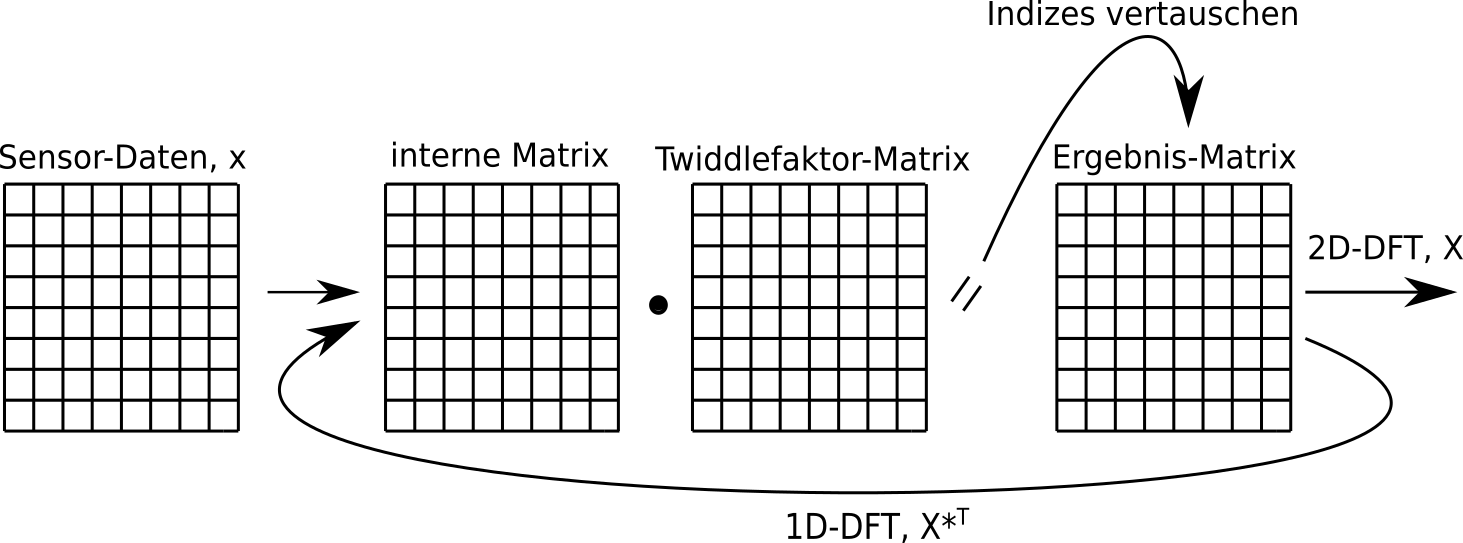
\includegraphics[width=0.95\textwidth]{img/MatMultTranspose2.png}
\end{figure}
\end{frame}
\restoreframe


\begin{frame}\frametitle{Berechnungsarten der DFT und deren Aufwand}
 \begin{itemize}
  \item optimierte Matrixmultiplikation mit reellen Eingangswerten
  \item optimierte Matrixmultiplikation mit komplexen Eingangswerten
  \item Fast Fouriertransformation (Butterfly-Algorithmus)
  \item allgemeine Matrixmultiplikation
 \end{itemize}
\end{frame}

% 1) Redundanzen der DFT, weniger Multiplikationen notwendig, Redundanz des Imaginärteils muss negiert werden
% 2) gleiche Einheit für 1D und 2D verwendbar, nur eine nötig
% 3) Transformationsart (-matrix) tauschbar
% 4) Vergleich, nicht von Interesse wegen ausschließlich $2^n$

\multipleframe
\begin{frame}\frametitle{2D-DFT mit reellen Eingangswerten zur Ausnutzung von Redundanzen}
\begin{minipage}{0.48\textwidth}
\begin{center}
 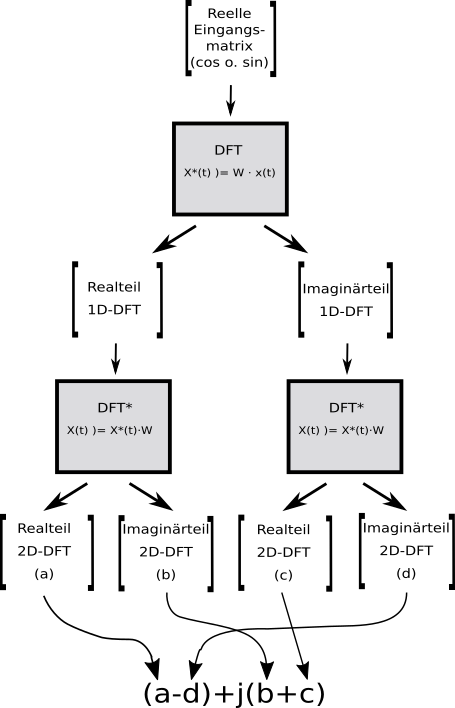
\includegraphics[width=0.85\textwidth]{img/reelleMatMult.png}
\end{center}
\end{minipage}
\hfill
\begin{minipage}{0.48\textwidth}
 
\end{minipage}
\end{frame}


\begin{frame}\frametitle{2D-DFT mit reellen Eingangswerten zur Ausnutzung von Redundanzen}
\begin{minipage}{0.48\textwidth}
\begin{center}
 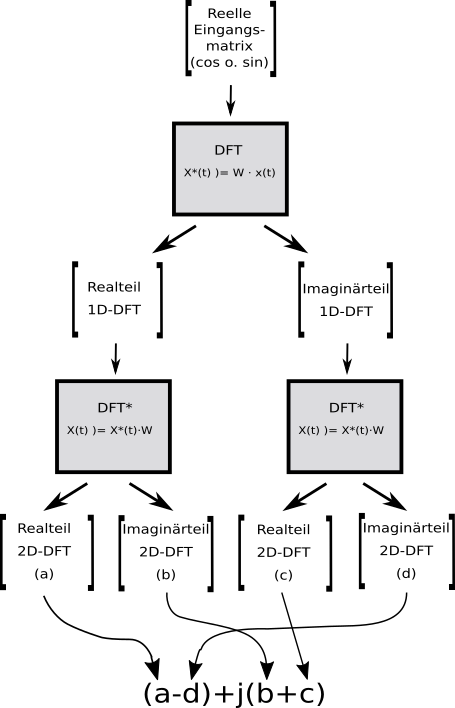
\includegraphics[width=0.85\textwidth]{img/reelleMatMult.png}
\end{center}
\end{minipage}
\hfill
\begin{minipage}{0.48\textwidth}
 \begin{center}
 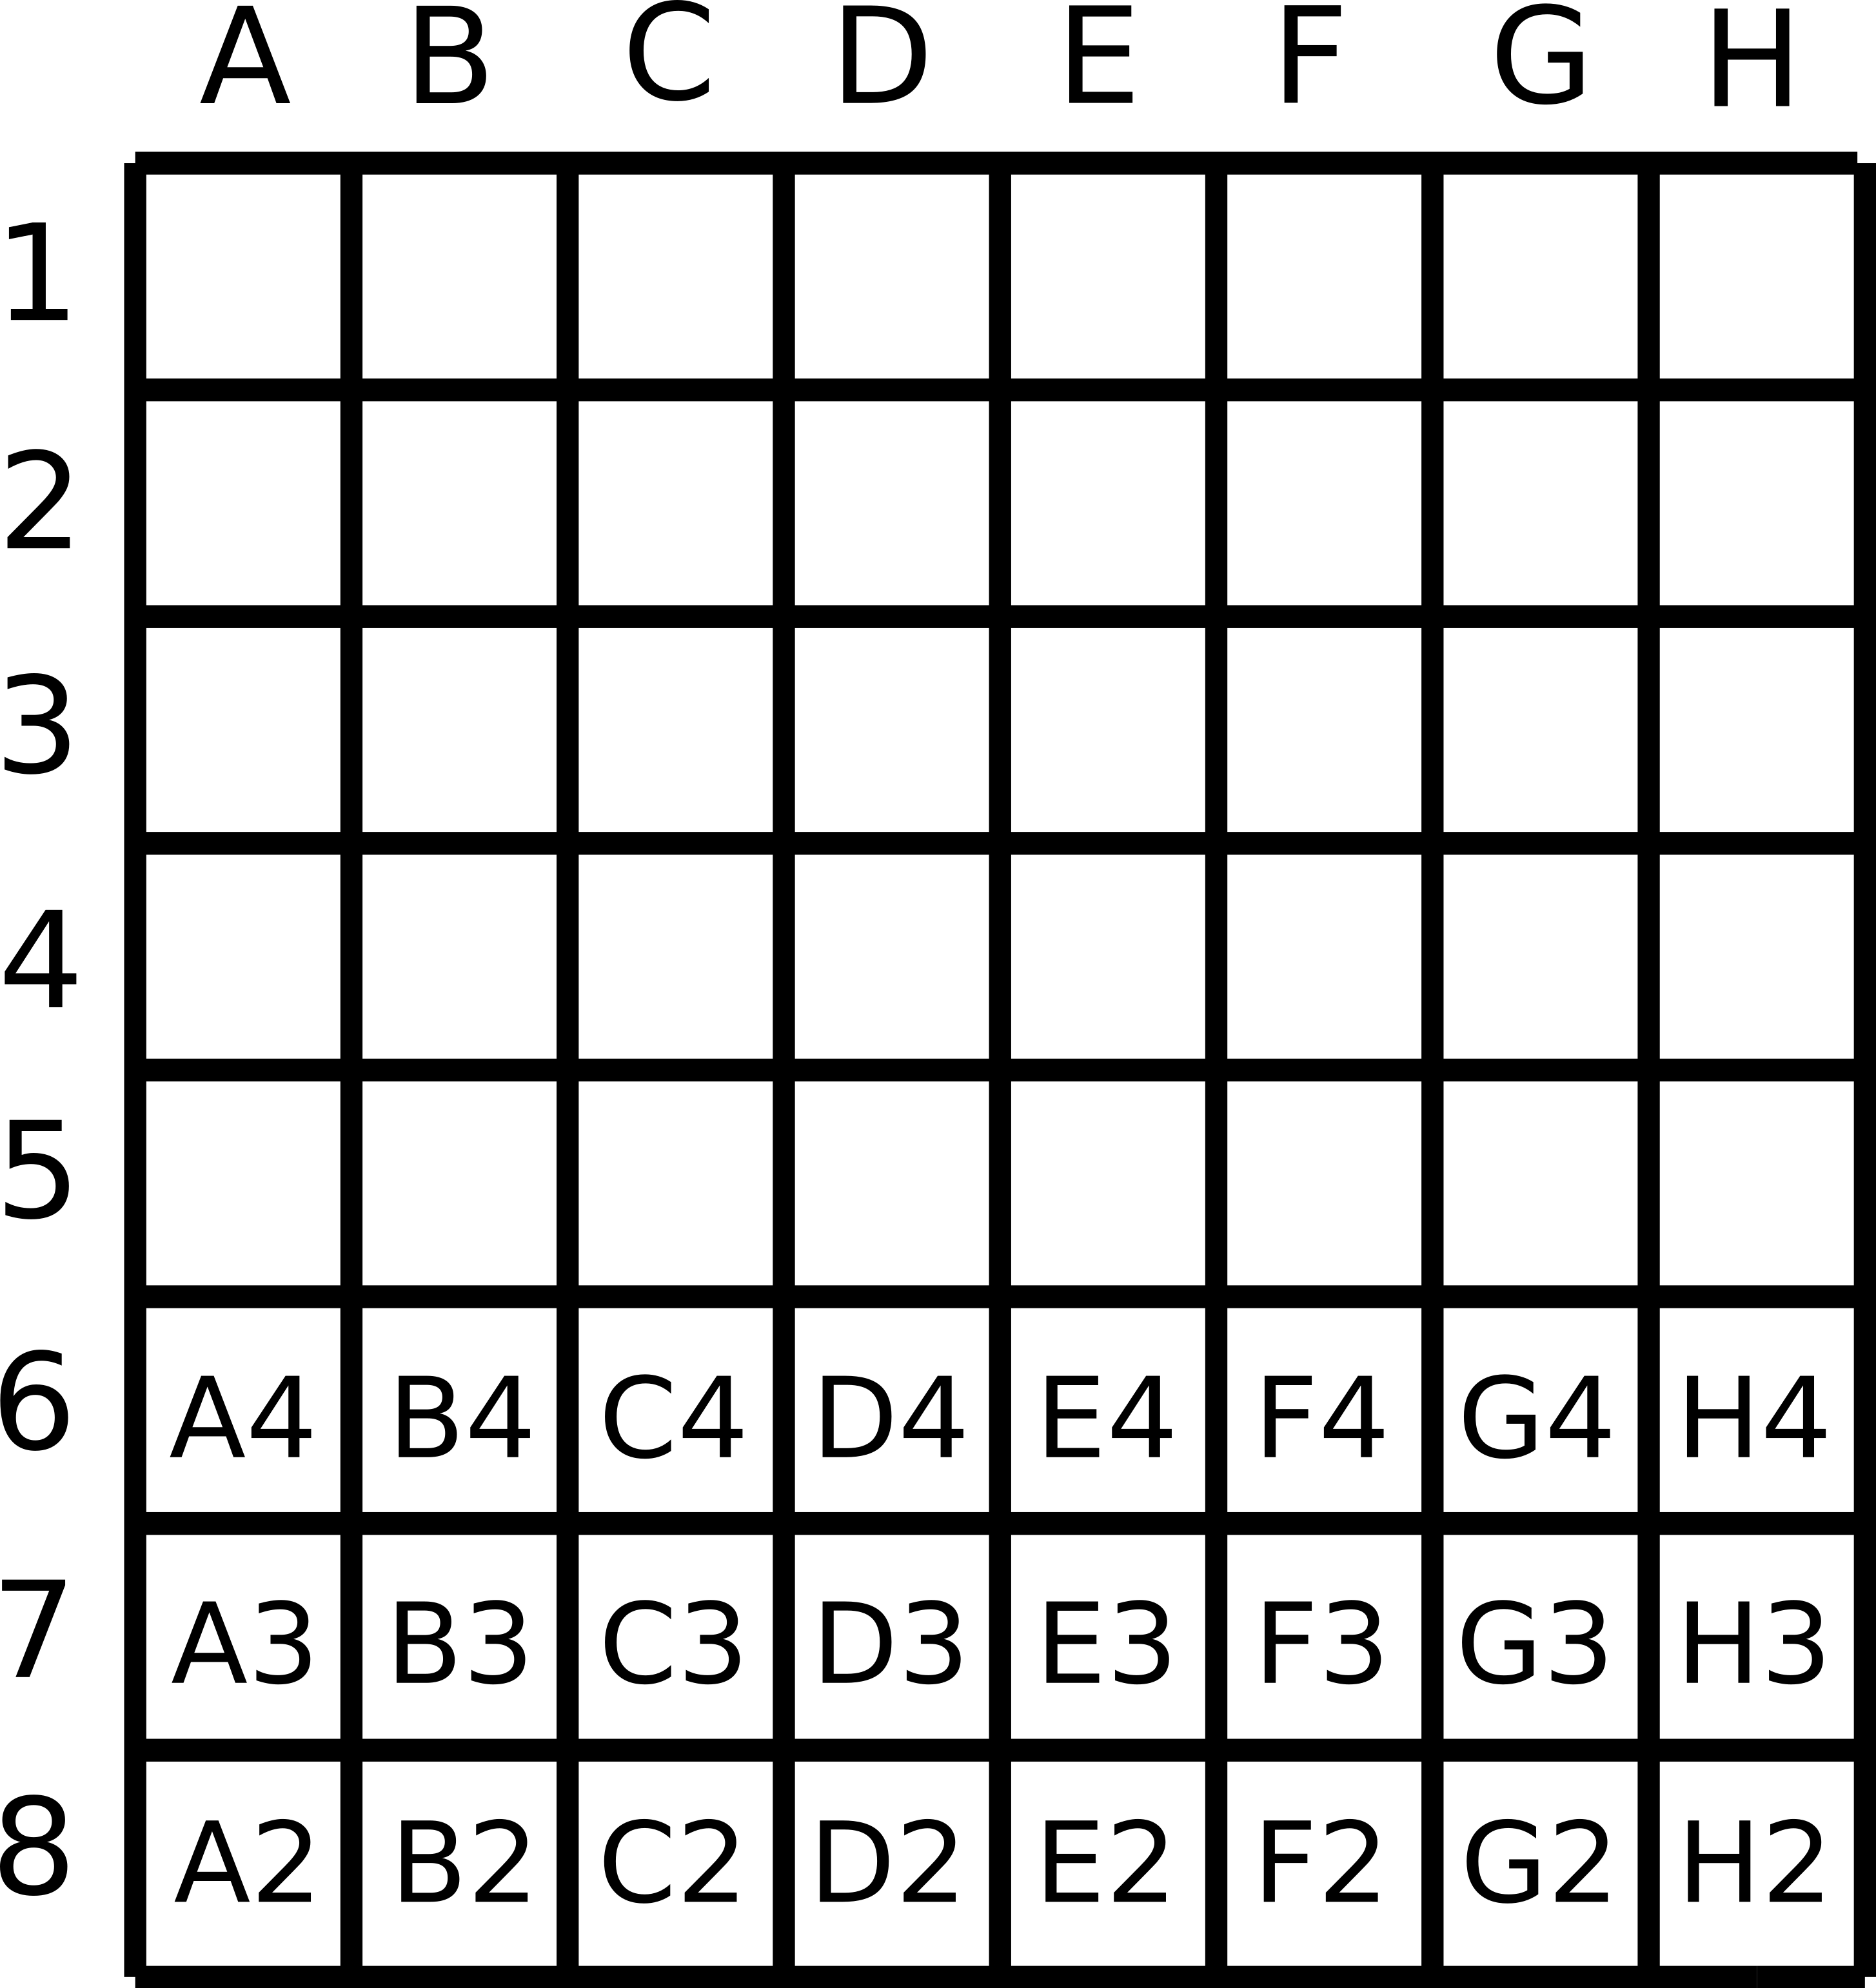
\includegraphics[width=0.6\textwidth]{img/reelleMatMultRedundanzRealteil.png} 
 
 \vspace{0.5cm}
 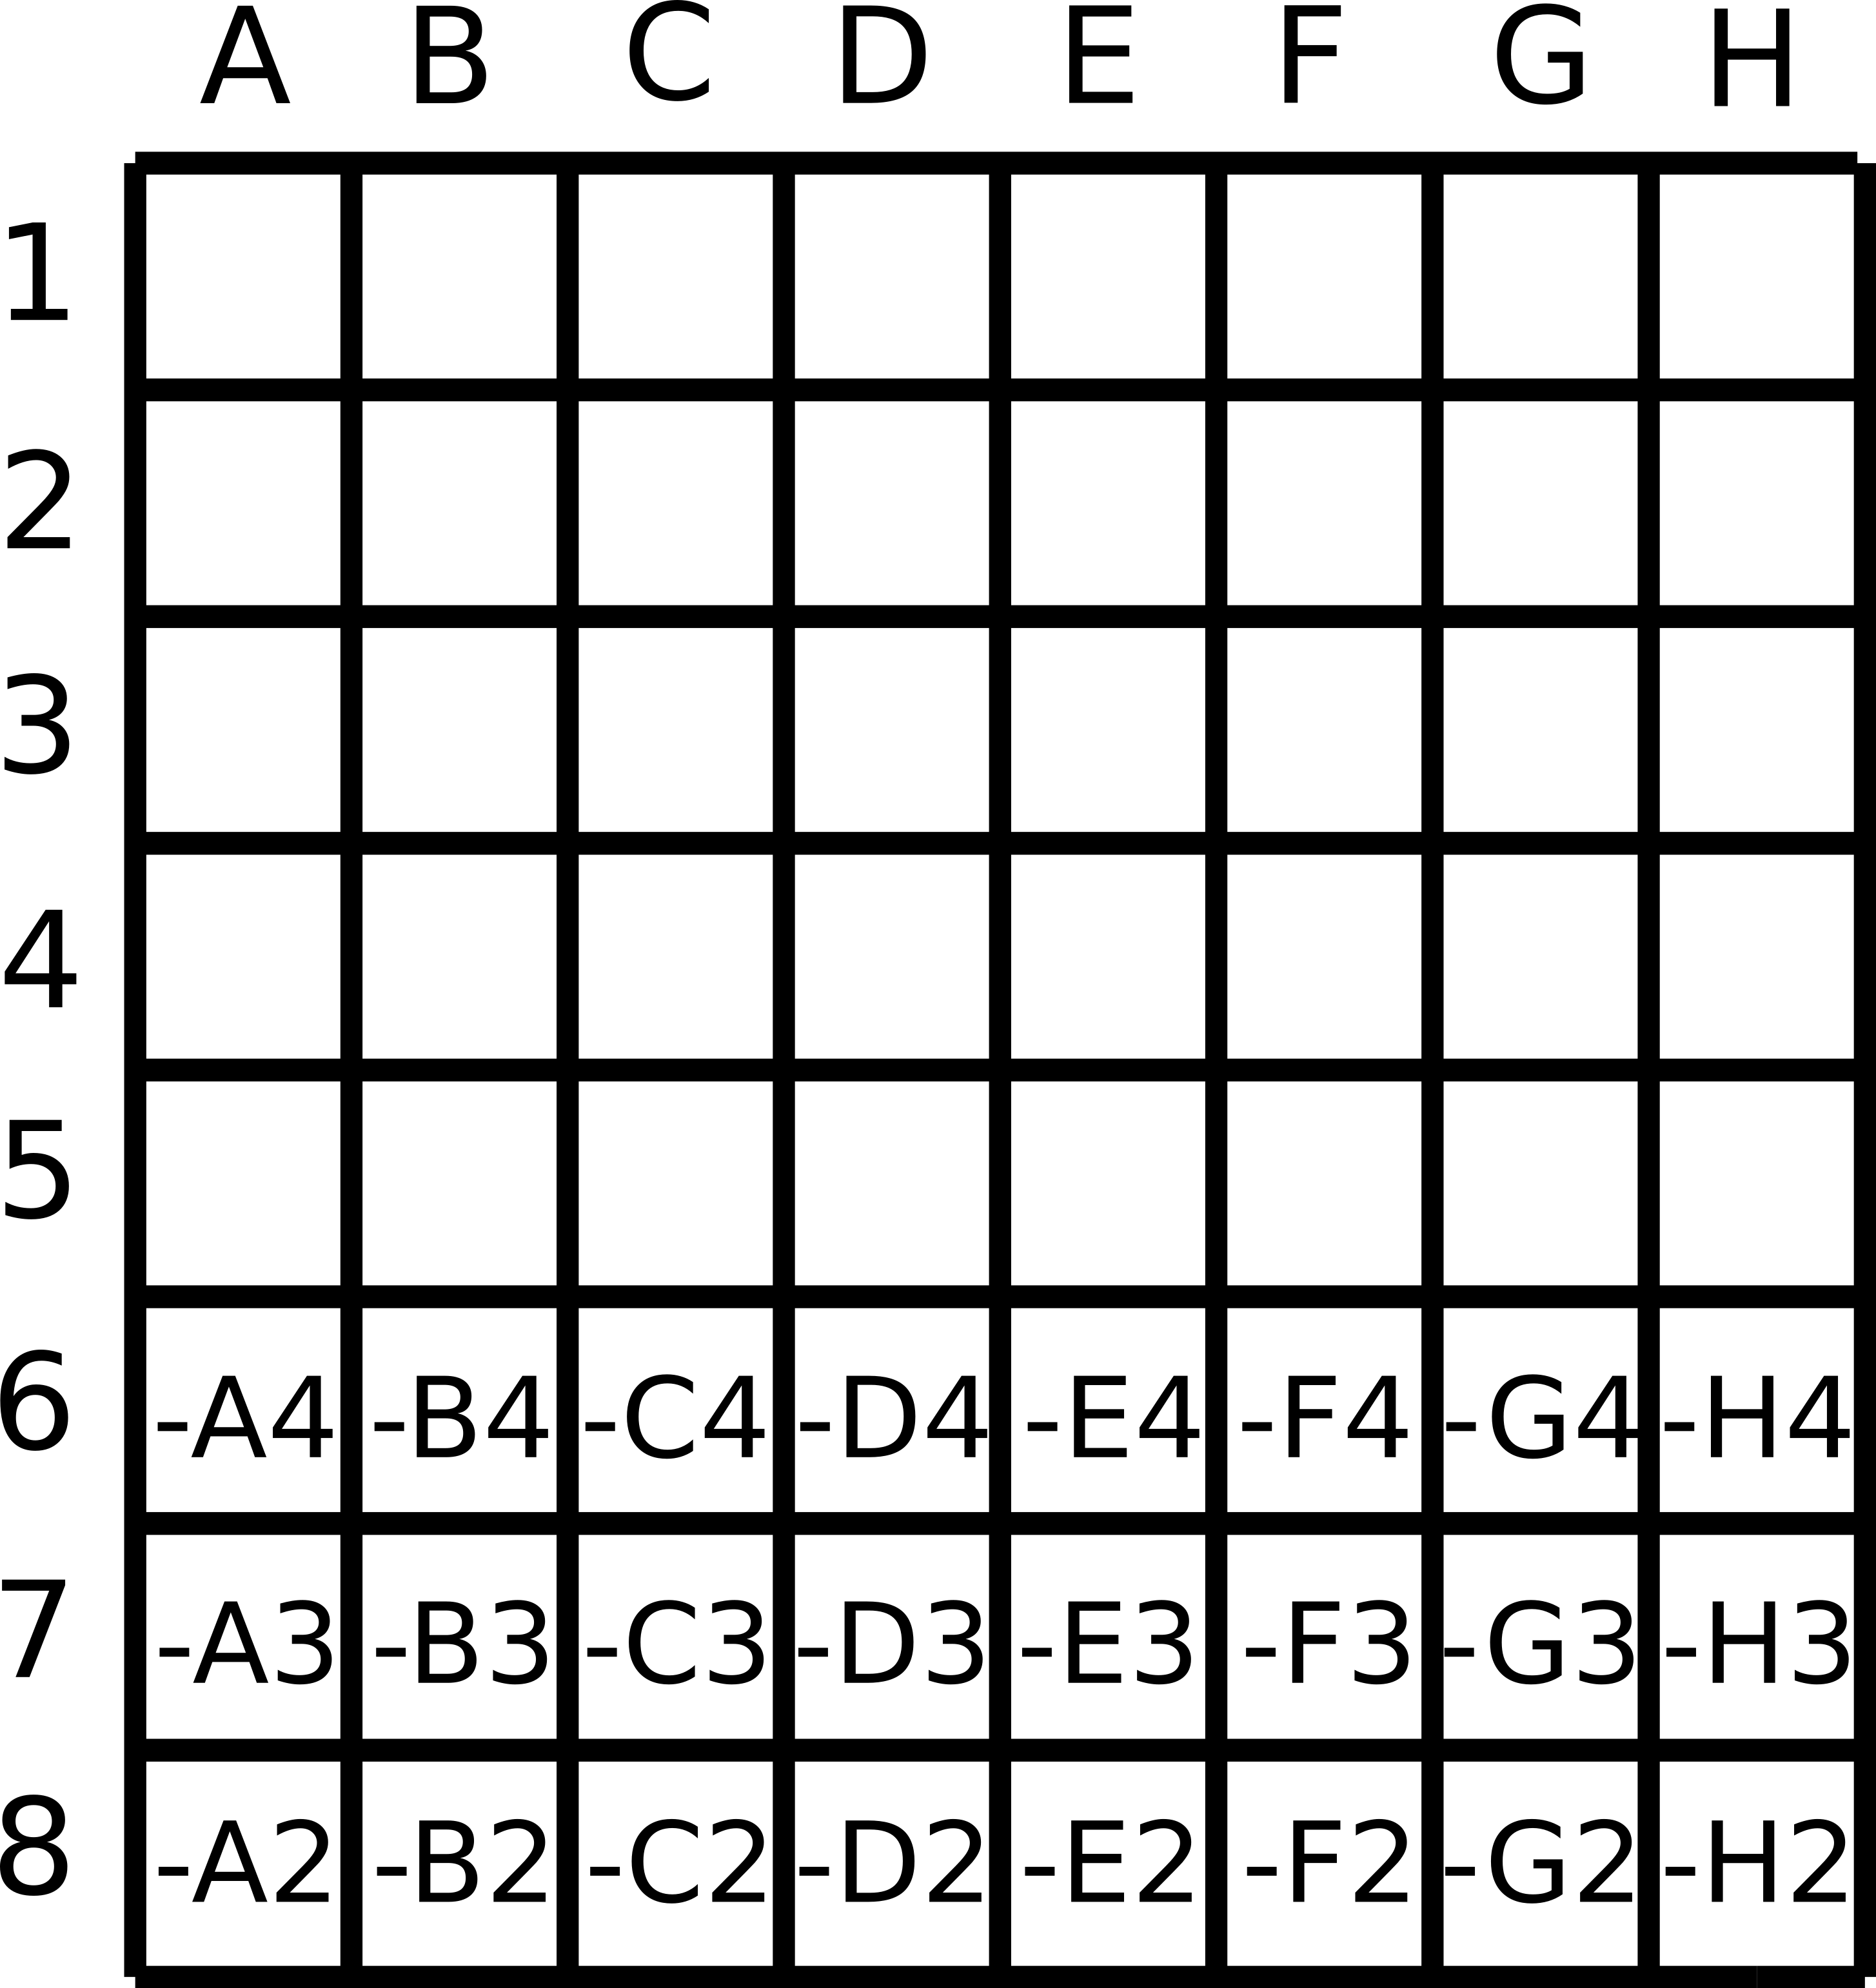
\includegraphics[width=0.6\textwidth]{img/reelleMatMultRedundanzImagteil.png} 
\end{center}
\end{minipage}
\end{frame}
\restoreframe


\begin{frame}\frametitle{2D-DFT mit komplexen Eingangswerten}
 \begin{figure}[htbp]
 \centering
   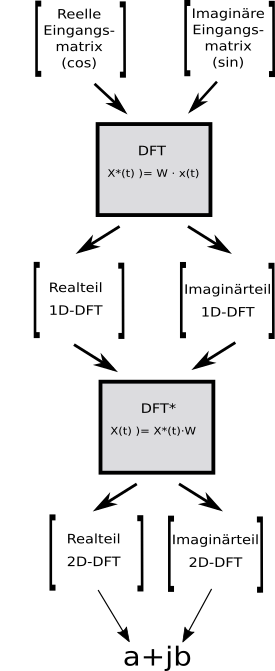
\includegraphics[width=0.25\textwidth]{img/komplexeMatMult.png}
% \caption{Veranschaulichung der Berechnung der DFT mit reellen Eingangswerten.}
 \label{pic:komplexeDFT}
\end{figure}
\end{frame}



\begin{frame}\frametitle{Anzahl reeller Multiplikationen für die Berechnung der 8x8-2D-DFT}

\begin{table}[ht!]
\centering
%\caption{Auflistung benötigter reeller Multiplikationen der verschiedenen Methoden für die 2D-DFT}
 \begin{tabular}{lc}
  \hline
  Methode  & Anzahl reeller Multiplikationen\\
  \hline
  reelle Eingangswerte   & 64\\
  komplexe Eingangswerte & 128\\
  FFT   & 128\\
  allgemeine Matrixmultiplikation & 4096\\
  \hline
 \end{tabular}
 \label{tab:AuflistungMultiplikationen}
\end{table} 
\end{frame}



\begin{frame}\frametitle{Analyse und Entwicklung}
Gliederung:
 \begin{itemize}
  \item Gegenüberstellung verschiedener Größen von Twiddlefaktormatrizen
  \item Optimieren der 8x8-DFT
  \item Konstantenmultiplikation
  \item Benötigte Takte
  \item Zustandsfolge
  \item Entwickeln der 2D-DFT auf Basis der 1D-DFT
 \end{itemize}

\end{frame}



\begin{frame}\frametitle{Gegenüberstellung verschiedener Größen von DFT-Twiddlefaktormatrizen}
  \begingroup
  \renewcommand*{\arraystretch}{1.2} % Zeilenabstand der Tabelle
  \begin{table}[!ht]
  \centering
   \begin{tabular}{lccccc}
   \hline
    N							& 8	& 9	& 12	& 15		& 16 \\
    \hline
    N$\times$N						& 64	& 81	& 144	& 225		& 256 \\
    \rowcolor{lightgray}
    trivial $\Re$ 					& 48	& 45	& 128	& 81		& 128 \\
    \rowcolor{lightgray}
    nicht triv. $\Re$					& 16	& 36	& 16	& 144		& 128 \\
    triv. $\Im$ 					& 48	& 21	& 96	& 45		& 128 \\
    nicht triv. $\Im$ 					& 16	& 60	& 48	& 180		& 128 \\
    \rowcolor{lightgray}
    $\sum$ triv. 					& 96	& 66	& 224	& 126		& 256 \\
    \rowcolor{lightgray}
    $\sum$ nicht triv. 					& 32	& 96	& 64	& 324		& 256 \\
    Anzahl verschiedener nicht trivialer Werte          & 1     & 7     & 1     & 13            & 3 \\
    Verhältnis  $\sum$ trivial / $\sum$ nicht trivial	& 3	& 0,6875& 3,5	& 0,3889	& 1\\
    \hline
   \end{tabular}
   \label{tab:DFT-TwiddlefaktorMatrizenBewertung}
  \end{table}
 \endgroup
 \vspace{1cm}
\end{frame}



\begin{frame}\frametitle{Optimierung der 8x8-DFT}
\vspace{0.3cm}
   \begin{figure}[!h]
  \centering
  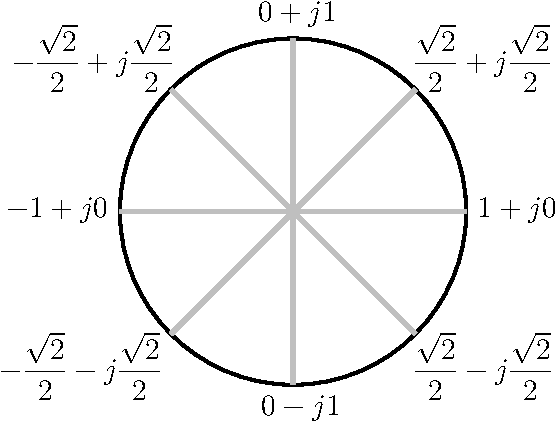
\includegraphics[width=0.3\textwidth]{img/Einheitskreis-crop.pdf}
\end{figure}

\vspace{-0.3cm}
\begin{center}
 \begin{minipage}{0.9\textwidth}
\begingroup
 %\renewcommand*{\arraystretch}{0.99} % Zeilenabstand der Tabelle

\begin{center}
  \[
   \stackrel{\mbox{$Re\{W\}$}}{
    \begin{bmatrix}
     \myboxOnePos 	& \myboxOnePos 		& \myboxOnePos 	& \myboxOnePos 		& \myboxOnePos 	& \myboxOnePos 		& \myboxOnePos 	& \myboxOnePos \\
     \myboxOnePos 	& \myboxSqrtPos 	& \myboxZero 	& \myboxSqrtNeg		& \myboxOneNeg	& \myboxSqrtNeg		& \myboxZero	& \myboxSqrtPos \\
     \myboxOnePos 	& \myboxZero 		& \myboxOneNeg 	& \myboxZero 		& \myboxOnePos 	& \myboxZero 		& \myboxOneNeg 	& \myboxZero \\
     \myboxOnePos 	& \myboxSqrtNeg 	& \myboxZero 	& \myboxSqrtPos 	& \myboxOneNeg 	& \myboxSqrtPos 	& \myboxZero 	& \myboxSqrtNeg \\
     \myboxOnePos 	& \myboxOneNeg 		& \myboxOnePos 	& \myboxOneNeg 		& \myboxOnePos 	& \myboxOneNeg 		& \myboxOnePos 	& \myboxOneNeg \\
     \myboxOnePos 	& \myboxSqrtNeg 	& \myboxZero 	& \myboxSqrtPos 	& \myboxOneNeg 	& \myboxSqrtPos 	& \myboxZero 	& \myboxSqrtNeg \\
     \myboxOnePos 	& \myboxZero 		& \myboxOneNeg 	& \myboxZero 		& \myboxOnePos 	& \myboxZero 		& \myboxOneNeg 	& \myboxZero \\
     \myboxOnePos 	& \myboxSqrtPos 	& \myboxZero 	& \myboxSqrtNeg		& \myboxOneNeg	& \myboxSqrtNeg		& \myboxZero	& \myboxSqrtPos 
    \end{bmatrix}
   }
   \hspace{1cm}
   \stackrel{\mbox{$Im\{W\}$}}{
    \begin{bmatrix}
     \myboxZero 	& \myboxZero 		& \myboxZero 	& \myboxZero 		& \myboxZero 	& \myboxZero 		& \myboxZero 	& \myboxZero \\
     \myboxZero 	& \myboxSqrtNeg 	& \myboxOneNeg 	& \myboxSqrtNeg		& \myboxZero	& \myboxSqrtPos		& \myboxOnePos	& \myboxSqrtPos \\
     \myboxZero 	& \myboxOneNeg 		& \myboxZero 	& \myboxOnePos 		& \myboxZero 	& \myboxOneNeg 		& \myboxZero 	& \myboxOnePos \\
     \myboxZero 	& \myboxSqrtNeg 	& \myboxOnePos 	& \myboxSqrtNeg 	& \myboxZero 	& \myboxSqrtPos 	& \myboxOneNeg 	& \myboxSqrtPos \\
     \myboxZero 	& \myboxZero 		& \myboxZero 	& \myboxZero 		& \myboxZero 	& \myboxZero 		& \myboxZero 	& \myboxZero \\
     \myboxZero 	& \myboxSqrtPos 	& \myboxOneNeg 	& \myboxSqrtPos		& \myboxZero 	& \myboxSqrtNeg 	& \myboxOnePos 	& \myboxSqrtNeg \\
     \myboxZero 	& \myboxOnePos 		& \myboxZero 	& \myboxOneNeg 		& \myboxZero 	& \myboxOnePos 		& \myboxZero 	& \myboxOneNeg \\
     \myboxZero 	& \myboxSqrtPos 	& \myboxOnePos 	& \myboxSqrtPos		& \myboxZero	& \myboxSqrtNeg		& \myboxOneNeg	& \myboxSqrtNeg 
    \end{bmatrix}
   }
  \]
\vspace{0.5cm}
  Legende: $\myboxOnePos$ = 1 \quad $\myboxOneNeg$ = -1 \quad $\myboxZero$ = 0 \quad $\myboxSqrtPos$ = $\nicefrac{\sqrt{2}}{2}$ \quad $\myboxSqrtNeg$ = -$\nicefrac{\sqrt{2}}{2}$
\end{center}
\endgroup
\end{minipage}
\end{center}

\end{frame}




\begin{frame}\frametitle{Anzahl benötigter Takte je Element, ungerade Zeilen}
 \begin{figure}
  \centering
  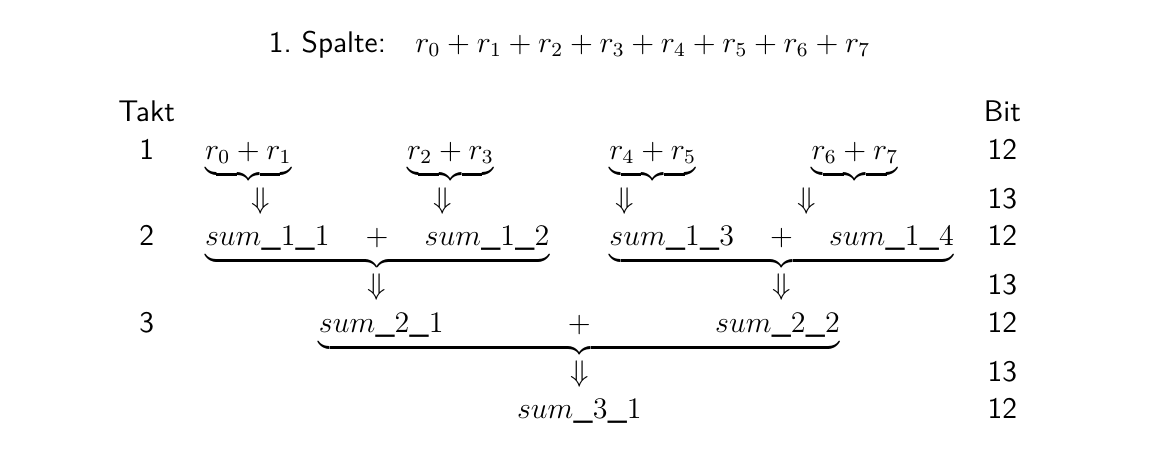
\includegraphics[width=0.9\textwidth]{img/ungeradeZeilen.png}
 \end{figure}
\end{frame}


\begin{frame}\frametitle{Anzahl benötigter Takte je Element, gerade Zeilen}
\begin{figure}
 \centering
 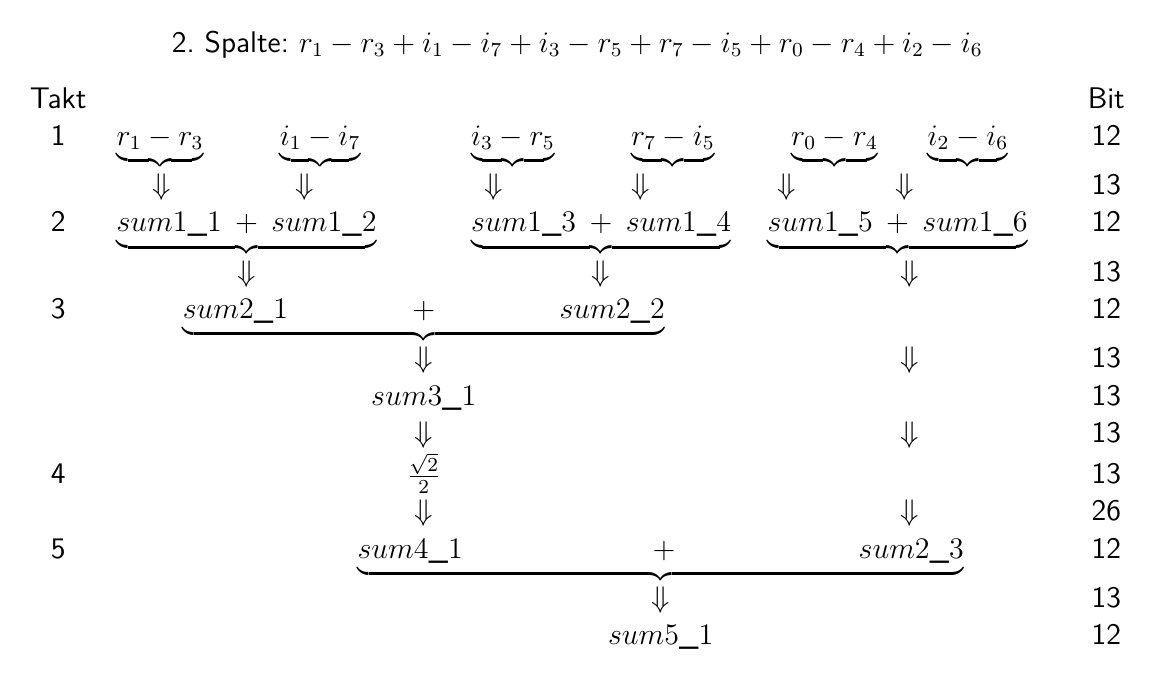
\includegraphics[width=0.9\textwidth]{img/geradeZeilen.png}
\end{figure}
\end{frame}


\begin{frame}\frametitle{Summe der Takte für die Berechnung der 2D-DFT}
\begin{table}[ht!]
\centering
%\caption{Benötigte Takte für die komplexe DFT}
%\label{tab:TakteKomplexeDFT}
\begin{tabular}{ccccc}
\hline
\multirow{2}{*}{Zeile} & Additionen & Takte pro Element & Takte für & Summe der\\
     & pro Element ($N$) & ($\log_2(N)$) & Multiplikation & Takte\\
\hline
1& 8  & 3   &0 &3\\
2& 12 & 3,6 &1 &5\\
3& 8  & 3   &0 &3\\
4& 12 & 3,6 &1 &5\\
5& 8  & 3   &0 &3\\
6& 12 & 3,6 &1 &5\\
7& 8  & 3   &0 &3\\
8& 12 & 3,6 &1 &5\\
\hline
\end{tabular}
\end{table}
\medskip
\begin{center}
$\Rightarrow$ Summe der Takte ist $\underbrace{(3 \cdot 4}_{\substack{\textrm{ungerade}\\\textrm{Zeilen}\\\textrm{aus}\\W}}  + \underbrace{5 \cdot 4)}_{\substack{\textrm{gerade}\\\textrm{Zeilen}\\\textrm{aus}\\W}} \cdot \underbrace{8}_{\substack{\textrm{alle}\\\textrm{Spalten}\\\textrm{aus}\\\textrm{Input}}} \cdot \underbrace{2}_{\substack{\textrm{1D-DFT}\\\textrm{und}\\\textrm{2D-DFT}}} = 512$ 
\end{center}
\end{frame}


\begin{frame}\frametitle{Konstantenmultiplikation mit $\frac{\sqrt{2}}{2} \simeq 0.70703125 = 0001011010100_2$}
 \begin{figure}[!ht]
\centering  
  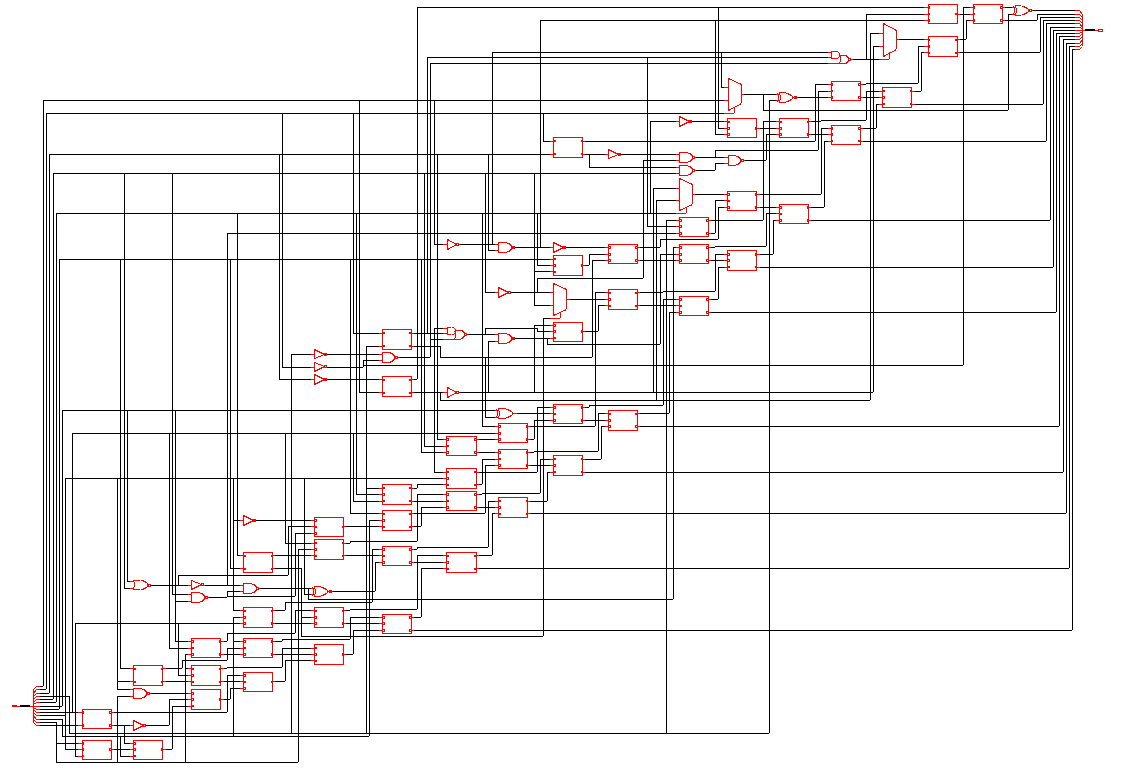
\includegraphics[width=1\textwidth]{img/13Bit_Konstantenmultiplizierer_neu.png}
\end{figure}
\end{frame}
% Gatter: 82 / 194
% Gater in Folge: 17
% Fläche: 6612 / 21985



% \begin{frame}\frametitle{Zustandsfolge}
%  \begin{figure}
%   \centering
%   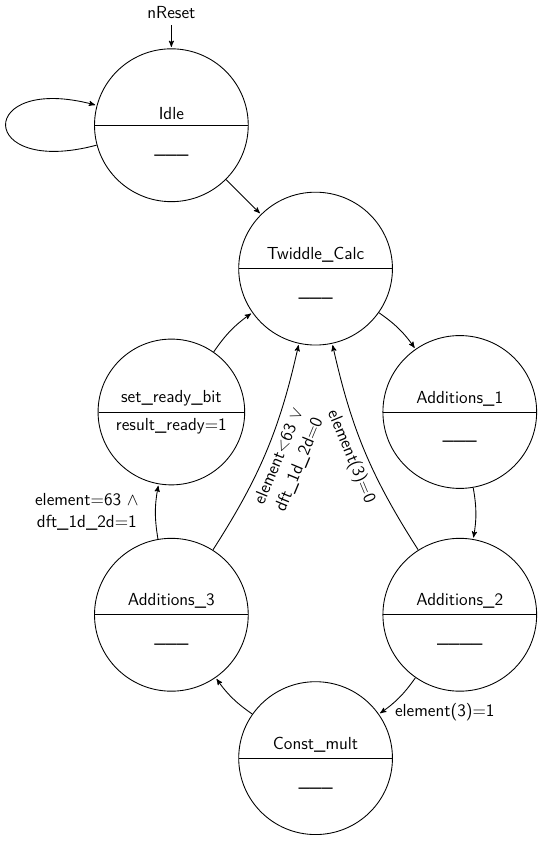
\includegraphics[width=0.45\textwidth]{img/Zustandsfolge.png}
%  \end{figure}
% \end{frame}




\begin{frame}\frametitle{Evaluation}
Gliederung:
 \begin{itemize}
  \item Testumgebung
  \item Zeitabschätzung
  \item Chipimplementation
 \end{itemize}

\end{frame}


\begin{frame}\frametitle{Testumgebung}
 \begin{itemize}
  \item Simulation mit NC\,Sim und SimVision
  \begin{itemize}
   \item nützlich für Teilfunktionen
   \item Betrachtung einzelner Signalverläufe
  \end{itemize}
  \item Automatisierung durch Shell-Skript
  \begin{itemize}
   \item Simulation mit NC\,Sim und TCL-Skript
   \item Berechnung mittels Matlab
   \item Vergleich
  \end{itemize}
 \end{itemize}
\end{frame}



\begin{frame}\frametitle{Simulationsprogramm NC\,Sim}
  \begin{figure}[htbp]
  \centering
  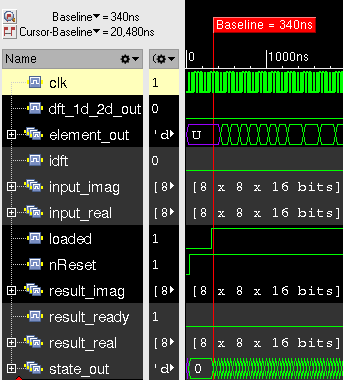
\includegraphics[width=0.58\textwidth]{img/Simulationsdauer_Anfang.png}
  \hfill
  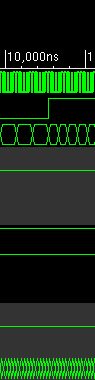
\includegraphics[width=0.161\textwidth]{img/Simulationsdauer_Mitte.png}
  \hfill
  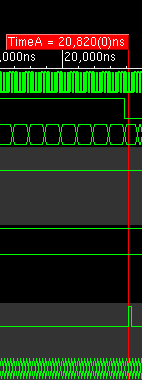
\includegraphics[width=0.241\textwidth]{img/Simulationsdauer_Ende.png}
 \end{figure}
\end{frame}

\begin{frame}\frametitle{Verifikation der benötigen Takte}
 \begin{figure}[htbp]
  \centering
  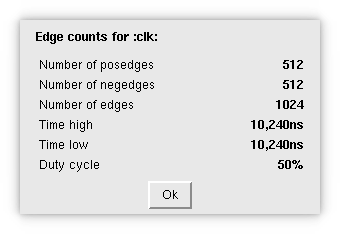
\includegraphics[width=0.6\textwidth]{img/Simulation_edge_count_clk.png}
 \end{figure}

\end{frame}



\begin{frame}\frametitle{Zeitabschätzung}
\vspace{-0.5cm}
\begin{center}
Gegeben: Systemtakt: \SI{100}{MHz}, max. Drehzahl: 8000min\,${}^{-1}$, Auflösung: $1^\circ$ 
\end{center}
\vspace{0.3cm}

 \begin{align*}
    \frac{8000\min^{-1}}{60} &= 1333,\bar{3}\,\texttt{sec}^{-1}  \\[10pt]
    \nonumber \curvearrowright 1\, \textrm{Umdrehung} &= \frac{1}{1333,\bar{3}\,\texttt{sec}^{-1}} = 7,5\cdot 10^{-3}\,\textrm{sec}\\[10pt]
    \nonumber 1^\circ &\widehat{=} \frac{7,5\cdot 10^{-3}\,\textrm{sec}}{360} = 20,83\cdot10^{-6}\,\sec \\[10pt]
    \textcolor{red}{20,83\cdot10^{-6}\sec \cdot 100\,\MHz} & \textcolor{red}{ = 2083\, \textrm{Takte}}
\end{align*}
\end{frame}


\begin{frame}\frametitle{Chipimplementation: Stromversorgung}
\begin{center}
        %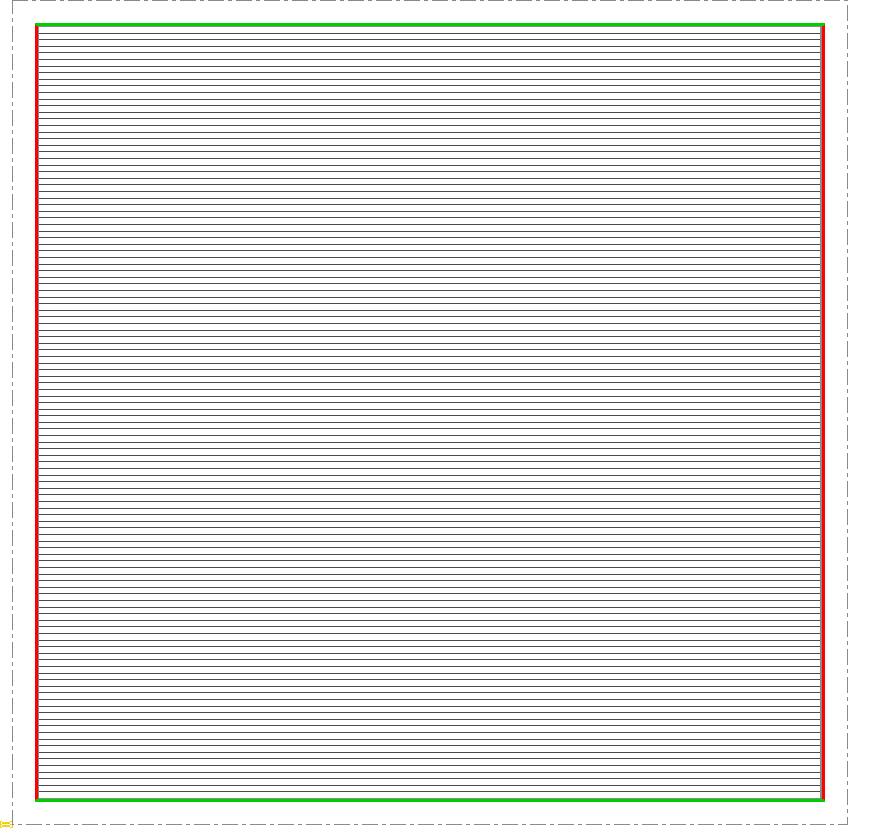
\includegraphics[width=0.35\textwidth]{img/FP_2.png}
        %\hfill
        %\quad
        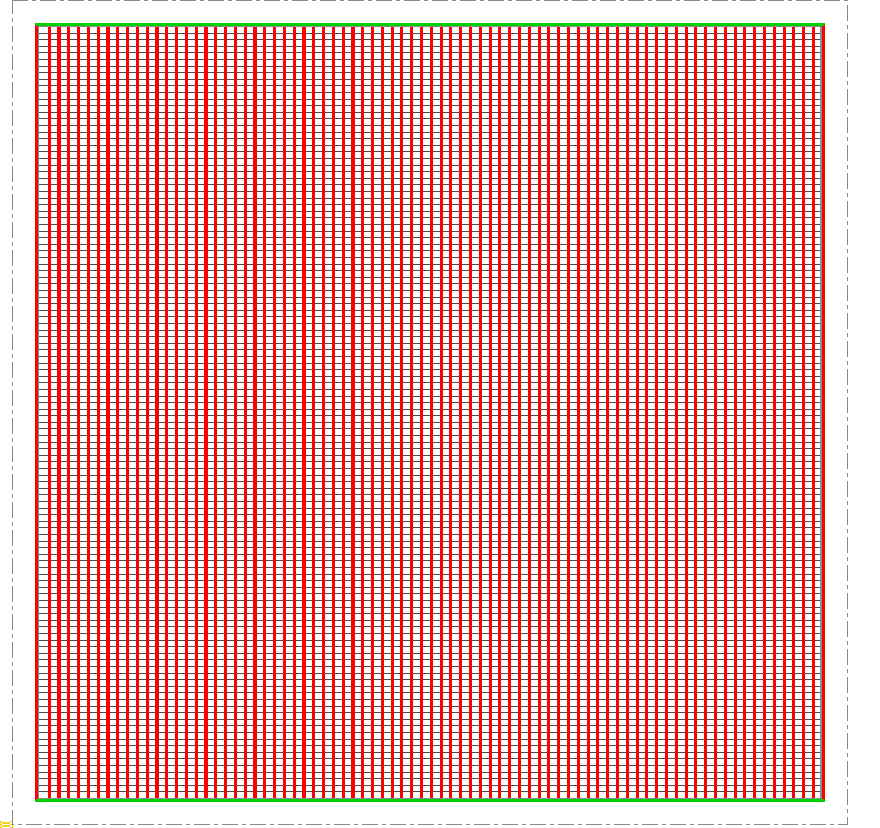
\includegraphics[width=0.49\textwidth]{img/FP_3.png}
        %\vskip\baselineskip
        \hfill
        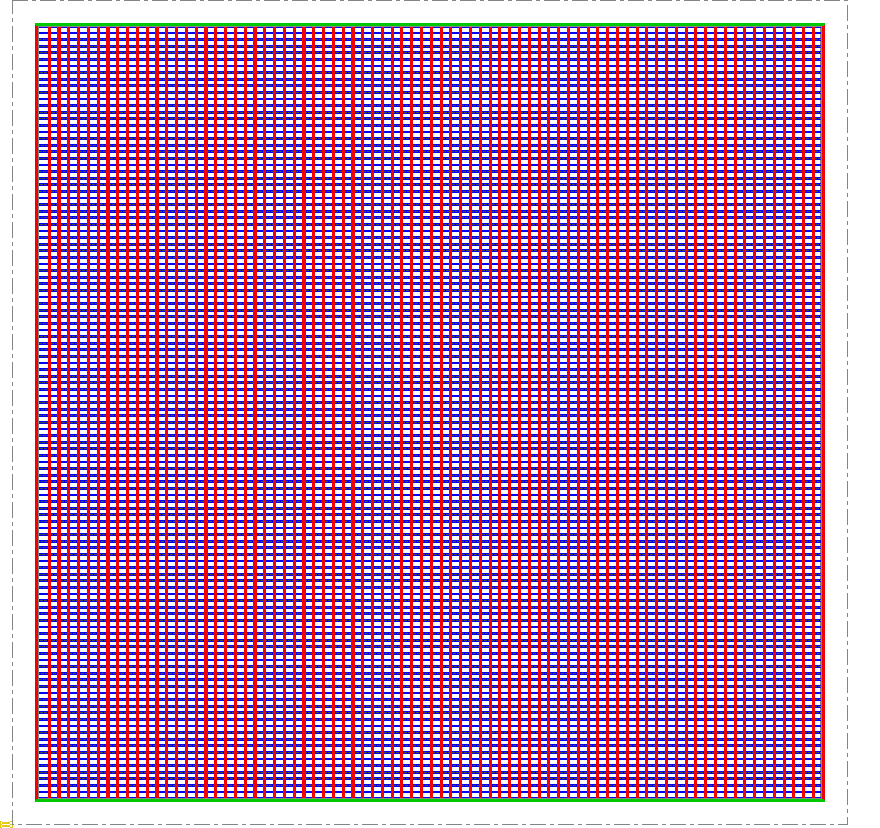
\includegraphics[width=0.49\textwidth]{img/FP_4.png}
        %\quad
        %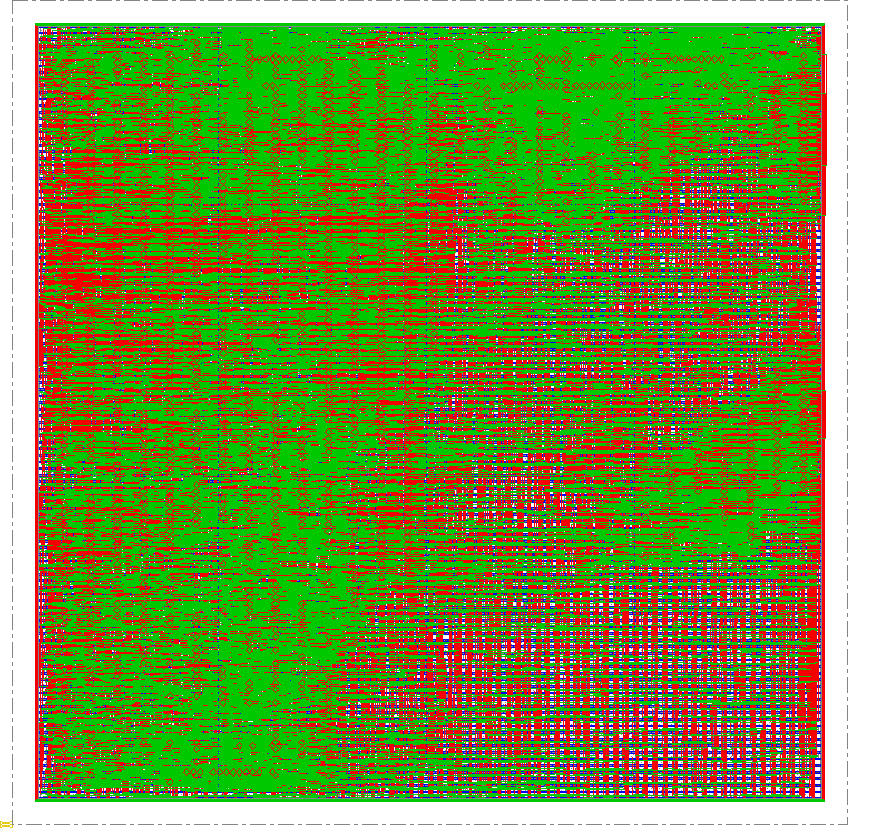
\includegraphics[width=0.35\textwidth]{img/FP_5.png}
        blau: Layer 1,  rot:  Layer 2,  grün: Layer 3
\end{center}
\end{frame}

\begin{frame}\frametitle{Chipimplementation: Platzierung der Standardzellen}
\begin{center}
 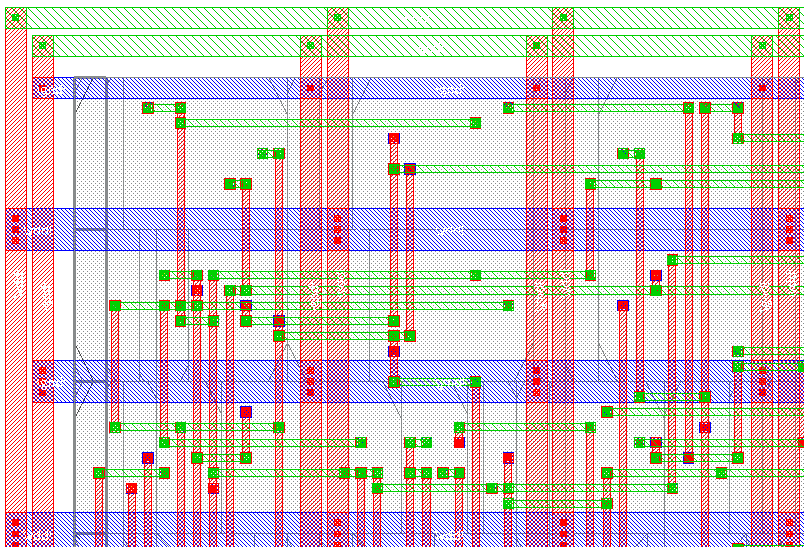
\includegraphics[width=0.85\textwidth]{img/Bilder/Screen1_BlockCell_crop_white.png}\\
 blau: Layer 1,  rot:  Layer 2,  grün: Layer 3
\end{center}
\end{frame}

\begin{frame}\frametitle{Chipimplementation: Platzierung der Standardzellen}
\begin{minipage}{0.69\textwidth}
 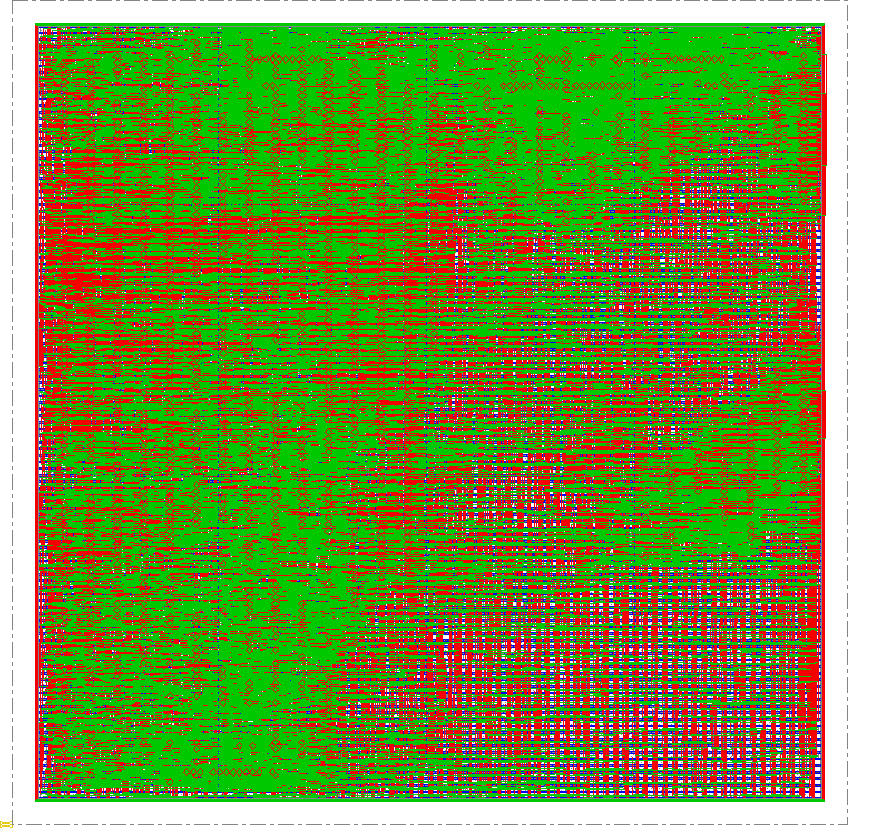
\includegraphics[width=1\textwidth]{img/FP_5.png}
\end{minipage}
\hfill%
\begin{minipage}{0.29\textwidth}
  Standardzellen:\\ \vspace{0.3cm}  \num{15310}\\
  Fläche:\\ \vspace{0.3cm} \num{1524960}µm² = 1,5mm²\\
  Prozess: \\ \vspace{0.3cm} 350µm²
\end{minipage}
\end{frame}










\multipleframe
\begin{frame}\frametitle{Zusatzfeature: Implementation der IDFT}

\begin{minipage}{0.48\textwidth}
\begin{minipage}{1\textwidth}

\begin{align*}
  W &= \sum_{m=0}^{N-1} \sum_{n=0}^{N-1} e^{\textcolor{red}{-}\frac{j 2 \pi m n}{N}}\\
\end{align*}
\end{minipage}

\begin{minipage}{1\textwidth}

\begin{center}
  %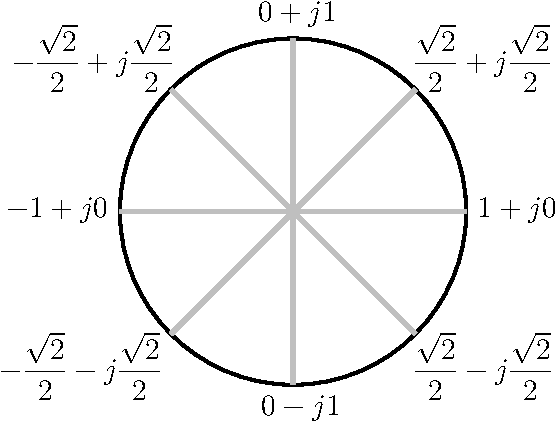
\includegraphics[width=0.6\textwidth]{img/Einheitskreis-crop.pdf}
\tikzstyle{dot}=[draw,shape=circle]

\begin{tikzpicture}[scale=1.2]
\draw[step=.5cm,gray, thin];
\draw (-1.2,0) -> (1.2,0);
\draw (0,-1.2) ->(0,1.2);
\draw (0,0) circle[radius=1cm];
\draw [thick] (0, 0) -- (0.866, 0.5);
\draw [thick] (0, 0) -- (0.866, -0.5);
\draw (1.1, 0.1) node {1};
\draw (1.3, 0.6) node {$e^{+j\pi kt}$};
\draw (1.3, -0.6) node {$e^{-j\pi kt}$};
\draw (-0.07, 1.2) node {$j$};
\draw (-1.2, 0.1) node {$-1$};
\draw (-0.2, -1.2) node {$-j$};
\node[dot, fill, inner sep=1pt] at(0.866,0.5){};
\node[dot, fill, inner sep=1pt] at(0.866,-0.5){};
\end{tikzpicture}

\end{center}
\end{minipage}
\end{minipage}
\hfill%
\begin{minipage}{0.48\textwidth}
\begin{minipage}{1\textwidth}
\begin{align*}
W^{*} &= \sum_{m=0}^{N-1} \sum_{n=0}^{N-1} e^{\textcolor{red}{+}\frac{j 2 \pi m n}{N}}\\
\end{align*} 
\end{minipage}
\begin{minipage}{1\textwidth}
\begin{center}

\includegraphics[width=0.6\textwidth]{img/IDFT_Zeilentausch_dummy.png}
\end{center}
\end{minipage}
\end{minipage}

\end{frame}

\begin{frame}\frametitle{Zusatzfeature: Implementation der IDFT}
\begin{minipage}{0.48\textwidth}
\begin{minipage}{1\textwidth}
\begin{align*}
  W &= \sum_{m=0}^{N-1} \sum_{n=0}^{N-1} e^{\textcolor{red}{-}\frac{j 2 \pi m n}{N}}\\
\end{align*}
\end{minipage}

\begin{minipage}{1\textwidth}
\begin{center}
  \tikzstyle{dot}=[draw,shape=circle]

\begin{tikzpicture}[scale=1.2]
\draw[step=.5cm,gray, thin];
\draw (-1.2,0) -> (1.2,0);
\draw (0,-1.2) ->(0,1.2);
\draw (0,0) circle[radius=1cm];
\draw [thick] (0, 0) -- (0.866, 0.5);
\draw [thick] (0, 0) -- (0.866, -0.5);
\draw (1.1, 0.1) node {1};
\draw (1.3, 0.6) node {$e^{+j\pi kt}$};
\draw (1.3, -0.6) node {$e^{-j\pi kt}$};
\draw (-0.07, 1.2) node {$j$};
\draw (-1.2, 0.1) node {$-1$};
\draw (-0.2, -1.2) node {$-j$};
\node[dot, fill, inner sep=1pt] at(0.866,0.5){};
\node[dot, fill, inner sep=1pt] at(0.866,-0.5){};
\end{tikzpicture}
\end{center}
\end{minipage}
\end{minipage}
\hfill%
\begin{minipage}{0.48\textwidth}
\begin{minipage}{1\textwidth}
\begin{align*}
W^{*} &= \sum_{m=0}^{N-1} \sum_{n=0}^{N-1} e^{\textcolor{red}{+}\frac{j 2 \pi m n}{N}}\\
\end{align*} 
\end{minipage}
\begin{minipage}{1\textwidth}
\begin{center}
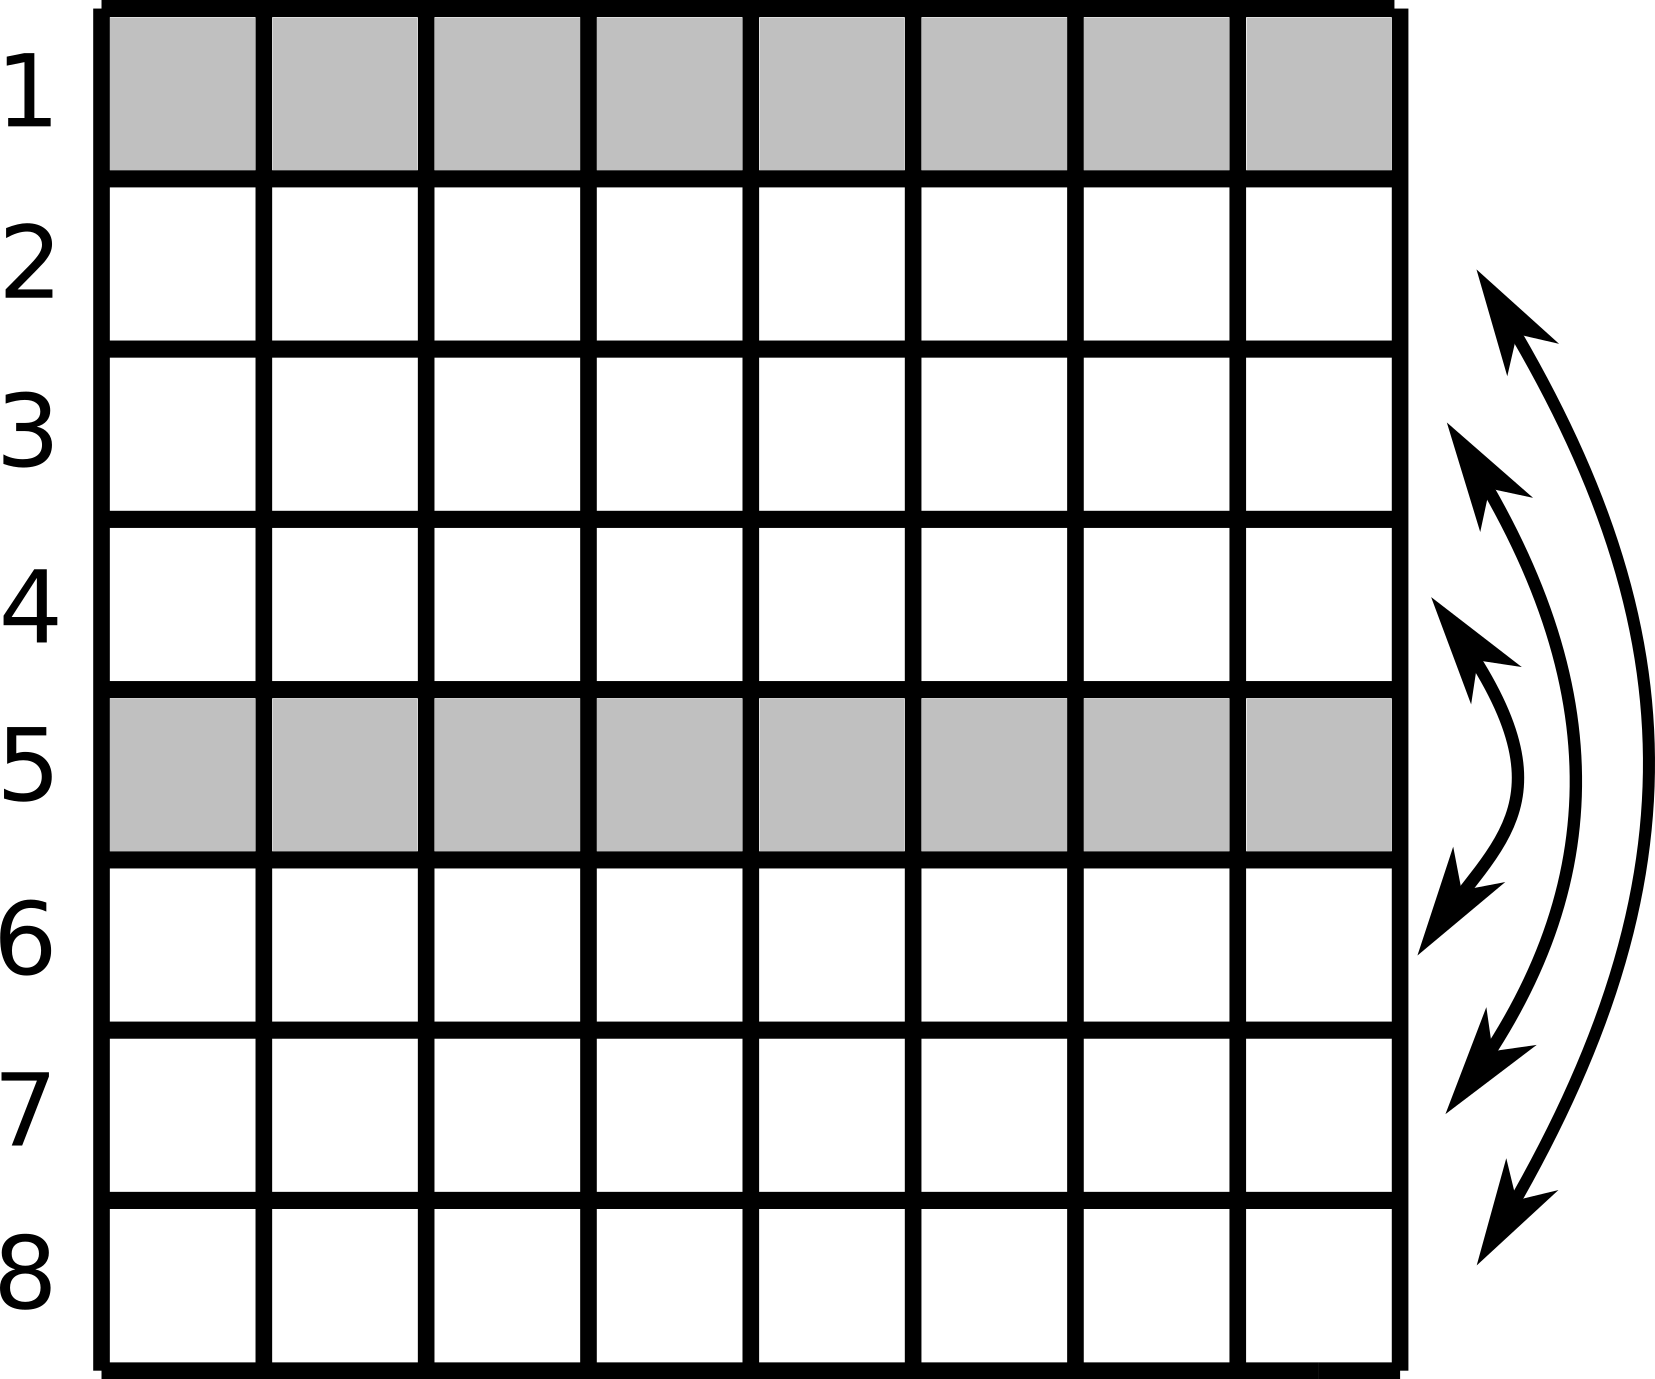
\includegraphics[width=0.6\textwidth]{img/IDFT_Zeilentausch.png}
\end{center}
\end{minipage}
\end{minipage}

\end{frame}
\restoreframe

\begin{frame}\frametitle{Zusammenfassung}
 \begin{itemize}
  \item DFT als 8x8 hat sich als effizient erwiesen
  \item Optimierung der Multiplikationen mit der Twiddlefaktormatrix
  \item Kritischer Pfad scheint Konstantenmultiplikation zu sein
  \item Berechnung der 1D- und 2D-DFT mit selber Einheit
  \item Benötigte Takte liegen im realistischen Rahmen
  \item DFT und IDFT benötigen zusammen etwa 50\% der verfügbaren Takte
  \item IDFT kann durch geringe Ergänzungen berechnet werden
  \item Wertvolle Grundlagen für die Implementation der 15x15 2D-DFT
 \end{itemize}

\end{frame}


\begin{frame}\frametitle{Ausblick}
\begin{itemize}
 \item Reduzierung des kritischen Pfades
 \begin{itemize}
  \item auf zwei Schaltnetze aufteilen
  \item Wallace-Tree verwenden
 \end{itemize}
 \item 15x15 mit ähnlich vielen Takten
\end{itemize}

 
\end{frame}


\end{document}

